\documentclass[11pt,a4paper]{article}
%\usepackage[utf8]{inputenc}
\usepackage{amsthm}
\usepackage{amsfonts}
\usepackage{amsmath}
\usepackage{amssymb}
\let\amssquare\square
\usepackage{mathtools}
%\usepackage{stmaryrd}
%\usepackage{tensor}
\usepackage[mathscr]{eucal}
\usepackage{url}
%\usepackage{marvosym}
\usepackage[left=2cm,right=2cm,top=2cm,bottom=2cm]{geometry}


\usepackage{tikz-cd}
\usetikzlibrary{positioning}
\usetikzlibrary{fit}
\usetikzlibrary{cd}
\usetikzlibrary{arrows}
\tikzset{ed/.style={auto,inner sep=2pt,font=\scriptsize}} %edges
\tikzset{>=stealth'}
\tikzset{vert/.style={draw,circle, minimum size=6mm, inner sep=0pt, fill=white}}
\tikzset{vertbig/.style={draw,circle, minimum size=8mm, inner sep=0pt, fill=white}}
%%% Add relative endpoints to curved 'to'

%% Due to limitations of TikZ, one cannot write '(a) to +(1,0)'.  The
%% target coordinate of a 'to' path must begin with a parenthesis.  In
%% this file we redefine the 'curve to' path to add options which
%% treat the target coordinate in a relative way.

%% With the option 'rel', the target coordinate is treated as if it
%% had a '+' in front of it, and similarly for 'rrel' and ++.  Note
%% that this can be misleading when reading the TikZ code if one is
%% unaware of its meaning, since we don't actually WRITE the + or ++
%% so the coordinate looks as if it were absolute.

%% The option 'abs' switches back to treating the target as absolute.

%% Ironically, these options DO NOT (yet) work together with the
%% 'relative' option (which calculates ANGLES relative to the line
%% from the source to the target coordinate).

\makeatletter

%%% Options to select relative endpoints
\newif\iftikz@to@relp
\tikz@to@relpfalse
\newif\iftikz@to@relpp
\tikz@to@relppfalse
\tikzoption{abs}[]{\tikz@to@relpfalse\tikz@to@relppfalse}
\tikzoption{rel}[]{\tikz@to@relptrue\tikz@to@relppfalse}
\tikzoption{rrel}[]{\tikz@to@relpfalse\tikz@to@relpptrue}


\tikzstyle{every curve to}=          []
\tikzstyle{curve to}=                [to path=\tikz@to@curve@path]

\tikzoption{bend angle}{\def\tikz@to@bend{#1}}

\tikzoption{bend left}[]{%
  \def\pgf@temp{#1}%
  \ifx\pgf@temp\pgfutil@empty%
  \else%
    \def\tikz@to@bend{#1}%
  \fi%
  \let\tikz@to@out=\tikz@to@bend%
  \c@pgf@counta=180\relax%
  \advance\c@pgf@counta by-\tikz@to@out\relax%
  \edef\tikz@to@in{\the\c@pgf@counta}%
  \tikz@to@switch@on%
  \tikz@to@relativetrue%
}

\tikzoption{bend right}[]{%
  \def\pgf@temp{#1}%
  \ifx\pgf@temp\pgfutil@empty%
  \else%
    \def\tikz@to@bend{#1}%
  \fi%
  % Now, negate
  \c@pgf@counta=\tikz@to@bend\relax%
  \c@pgf@counta=-\c@pgf@counta\relax%
  \edef\tikz@to@out{\the\c@pgf@counta}%
  \c@pgf@counta=180\relax%
  \advance\c@pgf@counta by-\tikz@to@out\relax%
  \edef\tikz@to@in{\the\c@pgf@counta}%
  \tikz@to@switch@on%
  \tikz@to@relativetrue%
}

\tikzoption{relative}[true]{\csname tikz@to@relative#1\endcsname}
\newif\iftikz@to@relative
\tikz@to@relativefalse

\tikzoption{in}{\def\tikz@to@in{#1}\tikz@to@switch@on}
\tikzoption{out}{\def\tikz@to@out{#1}\tikz@to@switch@on}

\tikzoption{in looseness}{\tikz@to@set@in@looseness{#1}}
\tikzoption{out looseness}{\tikz@to@set@out@looseness{#1}}
\tikzoption{looseness}{\tikz@to@set@in@looseness{#1}\tikz@to@set@out@looseness{#1}}

\tikzoption{in control}{\tikz@to@set@in@control{#1}}
\tikzoption{out control}{\tikz@to@set@out@control{#1}}
\tikzoption{controls}{\tikz@to@parse@controls#1\pgf@stop}

\tikzoption{in min distance}{\tikz@to@set@distances{#1}{}{}{}}
\tikzoption{in max distance}{\tikz@to@set@distances{}{#1}{}{}}
\tikzoption{in distance}{\tikz@to@set@distances{#1}{#1}{}{}}
\tikzoption{out min distance}{\tikz@to@set@distances{}{}{#1}{}}
\tikzoption{out max distance}{\tikz@to@set@distances{}{}{}{#1}}
\tikzoption{out distance}{\tikz@to@set@distances{}{}{#1}{#1}}
\tikzoption{min distance}{\tikz@to@set@distances{#1}{}{#1}{}}
\tikzoption{max distance}{\tikz@to@set@distances{}{#1}{}{#1}}
\tikzoption{distance}{\tikz@to@set@distances{#1}{#1}{#1}{#1}}

\def\tikz@to@set@distances#1#2#3#4{%
  \tikz@to@setifnotempy{#1}{\tikz@to@in@min}{\let\tikz@to@end@compute=\tikz@to@end@compute@looseness}%
  \tikz@to@setifnotempy{#2}{\tikz@to@in@max}{\let\tikz@to@end@compute=\tikz@to@end@compute@looseness}%
  \tikz@to@setifnotempy{#3}{\tikz@to@out@min}{\let\tikz@to@start@compute=\tikz@to@start@compute@looseness}%
  \tikz@to@setifnotempy{#4}{\tikz@to@out@max}{\let\tikz@to@start@compute=\tikz@to@start@compute@looseness}%
  \tikz@to@switch@on%
}

\def\tikz@to@setifnotempy#1#2#3{%
  \def\pgf@temp{#1}%
  \ifx\pgf@temp\pgfutil@empty\else\def#2{#1}#3\fi%
}


\def\tikz@to@set@in@looseness#1{%
  \def\tikz@to@in@looseness{#1}%
  \let\tikz@to@end@compute=\tikz@to@end@compute@looseness%
  \tikz@to@switch@on%
}
\def\tikz@to@set@out@looseness#1{%
  \def\tikz@to@out@looseness{#1}%
  \let\tikz@to@start@compute=\tikz@to@start@compute@looseness%
  \tikz@to@switch@on%
}

\def\tikz@to@parse@controls#1and#2\pgf@stop{\tikz@to@set@in@control{#2}\tikz@to@set@out@control{#1}}

\def\tikz@to@set@in@control#1{%
  \def\tikz@to@in@control{#1}%
  \let\tikz@to@end@compute=\tikz@to@end@compute@control%
  \tikz@to@switch@on%
}
\def\tikz@to@set@out@control#1{%
  \def\tikz@to@out@control{#1}%
  \let\tikz@to@start@compute=\tikz@to@start@compute@control%
  \tikz@to@switch@on%
}


\def\tikz@to@bend{30}

\def\tikz@to@out{45}
\def\tikz@to@in{135}

\def\tikz@to@out@looseness{1}
\def\tikz@to@in@looseness{1}

\def\tikz@to@in@min{0pt}
\def\tikz@to@in@max{10000pt}
\def\tikz@to@out@min{0pt}
\def\tikz@to@out@max{10000pt}

\def\tikz@to@switch@on{\let\tikz@to@path=\tikz@to@curve@path}

\def\tikz@to@curve@path{%
  [every curve to]
  \pgfextra{\iftikz@to@relative\tikz@to@compute@relative\else\tikz@to@compute\fi}
  \tikz@computed@path
  \tikztonodes%
  \pgfextra{\tikz@to@relpfalse\tikz@to@relppfalse}%
}

\def\tikz@to@modify#1#2{%
  \pgfutil@ifundefined{pgf@sh@ns@#1}
  {}%
  {\edef#1{#1.#2}}
}%

\def\tikz@to@compute{%
  \let\tikz@tofrom=\tikztostart%
  \let\tikz@toto=\tikztotarget%
  \tikz@to@modify\tikz@tofrom\tikz@to@out%
  \tikz@to@modify\tikz@toto\tikz@to@in%
  \ifx\tikz@to@start@compute\tikz@to@start@compute@looseness%
    \tikz@to@compute@distance%
  \else%
    \ifx\tikz@from@start@compute\tikz@to@start@compute@looseness%  
      \tikz@to@compute@distance%
    \fi%
  \fi%
  \tikz@to@start@compute%
  \tikz@to@end@compute%
  \iftikz@to@relp
    \edef\tikz@computed@path{.. controls \tikz@computed@start and \tikz@computed@end .. +(\tikz@toto)}
  \else
    \iftikz@to@relpp  
      \edef\tikz@computed@path{.. controls \tikz@computed@start and \tikz@computed@end .. ++(\tikz@toto)}
    \else
      \edef\tikz@computed@path{.. controls \tikz@computed@start and \tikz@computed@end .. (\tikz@toto)}
    \fi
  \fi
}

\def\tikz@to@compute@distance{\tikz@scan@one@point\tikz@@to@compute@distance(\tikz@tofrom)}
\def\tikz@@to@compute@distance#1{%
  \def\tikz@first@point{#1}%
  \iftikz@to@relp%
    \tikz@scan@one@point\tikz@@@to@compute@distance([shift={(\tikz@toto)}]\tikz@tofrom)%
  \else%
    \iftikz@to@relpp%
      \tikz@scan@one@point\tikz@@@to@compute@distance([shift={(\tikz@toto)}]\tikz@tofrom)%
    \else%
      \tikz@scan@one@point\tikz@@@to@compute@distance(\tikz@toto)%
    \fi%
  \fi}
\def\tikz@@@to@compute@distance#1{%
  \def\tikz@second@point{#1}%
  \tikz@to@compute@distance@main%
}
\def\tikz@to@compute@distance@main{%
  \pgf@process{\pgfpointdiff{\tikz@first@point}{\tikz@second@point}}%
  \ifdim\pgf@x<0pt\pgf@xa=-\pgf@x\else\pgf@xa=\pgf@x\fi%
  \ifdim\pgf@y<0pt\pgf@ya=-\pgf@y\else\pgf@ya=\pgf@y\fi%
  % 
  % Calculate length of second to first vector:
  % 
  \pgf@process{\pgfpointnormalised{\pgfqpoint{\pgf@xa}{\pgf@ya}}}%
  \ifdim\pgf@x>\pgf@y%
    \c@pgf@counta=\pgf@x%
    \ifnum\c@pgf@counta=0\relax%
    \else%
      \divide\c@pgf@counta by 255\relax%
      \pgf@xa=16\pgf@xa\relax%
      \divide\pgf@xa by\c@pgf@counta%
      \pgf@xa=16\pgf@xa\relax%
    \fi%
  \else%
    \c@pgf@counta=\pgf@y%
    \ifnum\c@pgf@counta=0\relax%
    \else%
      \divide\c@pgf@counta by 255\relax%
      \pgf@ya=16\pgf@ya\relax%
      \divide\pgf@ya by\c@pgf@counta%
      \pgf@xa=16\pgf@ya\relax%
    \fi%
  \fi%
  \pgf@x=0.3915\pgf@xa%
  \pgf@xa=\tikz@to@out@looseness\pgf@x%
  \pgf@xb=\tikz@to@in@looseness\pgf@x%
  % Adjust as necessary
  \pgfmathsetlength{\pgf@ya}{\tikz@to@out@min}
  \ifdim\pgf@xa<\pgf@ya%
    \pgf@xa=\pgf@ya%
  \fi%
  \pgfmathsetlength{\pgf@ya}{\tikz@to@out@max}
  \ifdim\pgf@xa>\pgf@ya%
    \pgf@xa=\pgf@ya%
  \fi%
  \pgfmathsetlength{\pgf@ya}{\tikz@to@in@min}
  \ifdim\pgf@xb<\pgf@ya%
    \pgf@xb=\pgf@ya%
  \fi%
  \pgfmathsetlength{\pgf@ya}{\tikz@to@in@max}
  \ifdim\pgf@xb>\pgf@ya%
    \pgf@xb=\pgf@ya%
  \fi%
}

\def\tikz@to@start@compute@looseness{%
  % Here, we can use the old version, since the source coordinate is
  % correct as-is.  Moreover, we need to, since using a relative first
  % control point doesn't work when the start coordinate is itself +
  % relative (it computes the control point relative to the previous
  % "current point").
  \edef\tikz@computed@start{([shift=(\tikz@to@out:\the\pgf@xa)]\tikz@tofrom)}%
%  \edef\tikz@computed@start{+(\tikz@to@out:\the\pgf@xa)}%
}
\def\tikz@to@end@compute@looseness{%
  % Here, we need to use a different version, since the target
  % coordinate is not necessarily being interpreted literally.
  % Fortunately, we are lucky and relative second control points seem
  % to always work.
  \edef\tikz@computed@end{+(\tikz@to@in:\the\pgf@xb)}%
%  \edef\tikz@computed@end{([shift=(\tikz@to@in:\the\pgf@xb)]\tikz@toto)}%
}
\def\tikz@to@start@compute@control{%
  \let\tikz@computed@start=\tikz@to@out@control%
}
\def\tikz@to@end@compute@control{%
  \let\tikz@computed@end=\tikz@to@in@control%
}

\let\tikz@to@start@compute=\tikz@to@start@compute@looseness%
\let\tikz@to@end@compute=\tikz@to@end@compute@looseness%




% Relative curves

\def\tikz@to@compute@relative{%
  \tikz@scan@one@point\tikz@@to@compute@relative(\tikztostart)%
}
\def\tikz@@to@compute@relative#1{%
  \def\tikz@tofrom{#1}%
  \tikz@scan@one@point\tikz@@@to@compute@relative(\tikztotarget)%
}
\def\tikz@@@to@compute@relative#1{%
  \def\tikz@toto{#1}%
  \begingroup
    % 
    % Adjust start and target so that they lie on the border in the
    % rotated coordinate system.
    %  
    \pgfutil@ifundefined{pgf@sh@ns@\tikztostart}
    {%
      \let\tikz@first@point=\tikz@tofrom%
      \let\tikz@tostart@tikz=\pgfutil@empty
    }%
    {%
      % Start computation of new start.
      {%
        \tikz@tofrom%
        \pgf@xc=\pgf@x%
        \pgf@yc=\pgf@y%
        {%
          \pgftransformreset%
          \pgftransformshift{\pgfqpoint{\pgf@xc}{\pgf@yc}}%
          \pgftransformrotate{\tikz@to@out}%
          \pgftransformshift{\pgfqpoint{-\pgf@xc}{-\pgf@yc}}%
          \pgf@process{\pgfpointtransformed{\tikz@toto}}%
        }%
        \pgf@xc=\pgf@x%
        \pgf@yc=\pgf@y%
        \pgfpointshapeborder{\tikztostart}{\pgfqpoint{\pgf@xc}{\pgf@yc}}%
        \xdef\tikz@tofrom@smuggle{\noexpand\pgfqpoint{\the\pgf@x}{\the\pgf@y}}
      }%
      \let\tikz@first@point=\tikz@tofrom@smuggle%
      \tikz@first@point%
      \edef\tikz@tostart@tikz{(\the\pgf@x,\the\pgf@y)}%
    }%
    \pgfutil@ifundefined{pgf@sh@ns@\tikztotarget}
    {%
      \let\tikz@second@point=\tikz@toto%
    }%
    {%
      % Start computation of new target.
      {%
        \tikz@toto%
        \pgf@xc=\pgf@x%
        \pgf@yc=\pgf@y%
        {%
          \pgftransformreset%
          \pgftransformshift{\pgfqpoint{\pgf@xc}{\pgf@yc}}%
          \pgftransformrotate{180}%
          \pgftransformrotate{\tikz@to@in}%
          \pgftransformshift{\pgfqpoint{-\pgf@xc}{-\pgf@yc}}%
          \pgf@process{\pgfpointtransformed{\tikz@tofrom}}%
        }%
        \pgf@xc=\pgf@x%
        \pgf@yc=\pgf@y%
        \pgfpointshapeborder{\tikztotarget}{\pgfqpoint{\pgf@xc}{\pgf@yc}}%
        \xdef\tikz@toto@smuggle{\noexpand\pgfqpoint{\the\pgf@x}{\the\pgf@y}}
      }%
      \let\tikz@second@point=\tikz@toto@smuggle%
    }%
    \tikz@second@point%
    \edef\tikz@totarget@tikz{(\the\pgf@x,\the\pgf@y)}%
    %
    % Compute distances
    %
    \tikz@to@compute@distance@main%
    \edef\tikz@to@first@distance{\the\pgf@xa}%
    \edef\tikz@to@second@distance{\the\pgf@xb}%
    %
    % Next step: Establish a transformed coordinate system so that the (modified)
    % start is at the origin and the (modified) target is at (1,0)
    %
    \pgftransformreset%
    \pgf@process{\tikz@first@point}%
    \pgf@xa=\pgf@x%
    \pgf@ya=\pgf@y%
    \pgf@process{\tikz@second@point}%
    \advance\pgf@x by-\pgf@xa%
    \advance\pgf@y by-\pgf@ya%
    \pgfpointnormalised{}%
    \pgf@xc=\pgf@x%
    \pgf@yc=\pgf@y%
    \pgf@xb=-\pgf@x%
    \pgf@yb=-\pgf@y%
    %
    % Now compute the control points.
    %
    {%
      \pgftransformshift{\tikz@first@point}%
      \pgftransformcm{\pgf@sys@tonumber\pgf@xc}{\pgf@sys@tonumber\pgf@yc}{\pgf@sys@tonumber\pgf@yb}{\pgf@sys@tonumber\pgf@xc}%
                      {\pgfpointorigin}%
      \pgf@process{\pgfpointtransformed{\pgfpointpolar{\tikz@to@out}{\tikz@to@first@distance}}}%
      \xdef\tikz@computed@start{(\the\pgf@x,\the\pgf@y)}%
    }
    {%
      \pgftransformshift{\tikz@second@point}%
      \pgftransformcm{\pgf@sys@tonumber\pgf@xc}{\pgf@sys@tonumber\pgf@yc}{\pgf@sys@tonumber\pgf@yb}{\pgf@sys@tonumber\pgf@xc}%
                      {\pgfpointorigin}%
      \pgf@process{\pgfpointtransformed{\pgfpointpolar{\tikz@to@in}{\tikz@to@second@distance}}}%
      \xdef\tikz@computed@end{(\the\pgf@x,\the\pgf@y)}%
    }
    \xdef\tikz@computed@path{
      \tikz@tostart@tikz
      .. controls \tikz@computed@start and \tikz@computed@end ..
      \tikz@totarget@tikz}%
  \endgroup
}


\theoremstyle{plain}
\newtheorem{theorem}{Theorem}[subsection]
%\newtheorem{axiom}[theorem]{Axiom}
\newtheorem*{theoremstar}{Theorem}
%\newtheorem{fact}[theorem]{Fact}
\newtheorem{proposition}[theorem]{Proposition}
\newtheorem{lemma}[theorem]{Lemma}
\newtheorem{corollary}[theorem]{Corollary}

\theoremstyle{definition}
\newtheorem{definition}[theorem]{Definition}
%\newtheorem{convention}[theorem]{Convention}
%\newtheorem{construction}[theorem]{Construction}
\newtheorem{example}[theorem]{Example}
%\newtheorem{examples}[theorem]{Examples}
%\newtheorem{notation}[theorem]{Notation}
\newtheorem{remark}[theorem]{Remark}
%\newtheorem{idea}[theorem]{Idea}
%\newtheorem{question}[theorem]{Question}

\newcommand{\C}{\mathscr{C}}
\newcommand{\homC}{\underline{\C}}
\newcommand{\D}{\mathscr{D}}
\newcommand{\E}{\mathscr{E}}
\newcommand{\M}{\mathscr{M}}
\newcommand{\N}{\mathscr{N}}
\newcommand{\T}{\mathscr{T}}

\newcommand{\bN}{\mathbb{N}}
\newcommand{\bZ}{\mathbb{Z}}


\newcommand{\Pastro}{\Phi}
%\newcommand{\Pastro}{\mathrm{Pastro}}
\newcommand{\Double}{\mathcal{D}}

% Categories
\newcommand{\Set}{\mathbf{Set}}
\newcommand{\Cat}{\mathbf{Cat}}
\newcommand{\Prof}{\mathbf{Prof}}
\newcommand{\MonCat}{\mathbf{MonCat}}
\newcommand{\LaxMonCat}{\mathbf{LaxMonCat}}
\newcommand{\SymmMonCat}{\mathbf{SymmMonCat}}
\newcommand{\Tele}{\mathbf{Tele}}

\newcommand{\Act}{\mathbf{Act}}
\newcommand{\Optic}{\mathbf{Optic}}
\newcommand{\Lawful}{\mathbf{Lawful}}
\newcommand{\SemiOptic}{\mathbf{SemiOptic}}
\newcommand{\Lens}{\mathbf{Lens}}
\newcommand{\Prism}{\mathbf{Prism}}
\newcommand{\Setter}{\mathbf{Setter}}
\newcommand{\Hask}{\mathbf{Hask}}
\newcommand{\Endo}{\mathbf{Endo}}
\newcommand{\Strong}{\mathbf{Strong}}
\newcommand{\Tamb}{\mathbf{Tamb}}
\newcommand{\Point}{\mathbf{Point}}
\newcommand{\CoPoint}{\mathbf{CoPoint}}
\newcommand{\Traversable}{\mathbf{Traversable}}

\newcommand{\id}{\mathrm{id}}
\newcommand{\op}{\mathrm{op}}
\newcommand{\const}{\mathrm{const}}
\DeclareMathOperator{\ob}{ob}
\DeclareMathOperator{\copr}{copr}
\newcommand{\inl}{\mathrm{inl}}
\newcommand{\inr}{\mathrm{inr}}
\DeclareMathOperator{\im}{im}

\newcommand{\fget}{\textsc{Get}}
\newcommand{\fput}{\textsc{Put}}
\newcommand{\fmodify}{\textsc{Modify}}
\newcommand{\freview}{\textsc{Review}}
\newcommand{\fmatching}{\textsc{Matching}}

% Special arrows
\newcommand{\isoto}{\xrightarrow{\cong}}
\newcommand{\hto}{\ensuremath{\,\mathaccent\shortmid\rightarrow\,}}

\makeatletter
\providecommand{\leftsquigarrow}{%
  \mathrel{\mathpalette\reflect@squig\relax}%
}
\newcommand{\reflect@squig}[2]{%
  \reflectbox{$\m@th#1\rightsquigarrow$}%
}
\makeatother

% Draft helpers
\newcommand{\todo}[1]{\textcolor{red}{\small #1}}

\newif\ifhideproofs
%\hideproofstrue %uncomment to hide proofs
\ifhideproofs
\usepackage{environ}
\NewEnviron{hide}{}
\let\proof\hide
\let\endproof\endhide
\fi

\title{Categories of Optics}
\author{Mitchell Riley}
\begin{document}
\maketitle

\section{Introduction}

\todo{TODO: Might have to adjust the entire thing because the action of $\M$ on $\C$ is not strictly monoidal. On the other hand, through the entire Pastro/Street paper pretends associativity/etc is strict, so maybe who cares? What we really want is just a (non-strict) monoidal functor $\M \to [\C, \C]$ from some $\M$. I may also want to put $\otimes$ and $\cdot$ everywhere instead of just writing $MA$ and $NMA$.}

\todo{Past work:
\begin{itemize}
\item The Haskell lens people: edwardk, shachaf, xplat, roconnor... (TODO: find out who these people are)
\item The Doubles paper
\item Bartosz's blog post which was written about the same time I started this. (Only tensor-like optics, no discussion of laws, confusion about enrichment(?))
\item The profunctor optics paper out of Oxford. (No generality, nothing categorical, no discussion of laws)
\end{itemize}
}

\todo{Contributions:
\begin{itemize}
\item ...
\end{itemize}
}

\todo{Introduction should include:
\begin{itemize}
\item Previous attempts to generalise optics
\item Some remark about how it's hard to isolate exactly what $\Set$-like properties are being used
\end{itemize}
}
A lens from $S$ to $A$ is a pair of maps $\fget : S \to A$ and $\fput : S \times A \to S$ that typically obeys three laws (whose names are in diagrammatic order):
\begin{itemize}
\item ``$\fput\fget$'': $\fget \; \fput = \pi_2$ as maps $S \times A \to A$, so that any update to $A$ should be \todo{represented faithfully in $S$},
\item ``$\fget\fput$'': $\fput [\id_S, \fget] = \id_S$ as maps $S \to S$, so that if $A$ is not changed then $S$ should not change; and,
\item ``$\fput\fput$'': $\fput (\fput \times \id_A) = \fput \, \pi_{1, 3}$ as maps $S \times A \times A \to S$, so any update to $A$ completely overwrites previous updates.
\end{itemize}

\todo{talk about ``constant complement'' idea}

\subsection{Notation}
\todo{I am open to changing any/all of these}
\begin{itemize}
\item Given $f : A \to B$ and $g : A \to C$, I write $[f, g] : A \to B \times C$ and $!_A : A \to 1$.
\item Given $f : A \to B$ and $g : C \to D$, I write $f \times g : A \times C \to B \times D$.
\item Given a $x \in P(C, C)$, I write $\langle x \rangle \in \int^C P(C, C)$ for its image, and $\copr_C : P(C,C) \to \int^C P(C, C)$
\item For a monoidal category, the structure maps are $\alpha$, $\lambda$ and $\rho$. A symmetry is $s$.
\end{itemize}

\todo{
\subsection{(Co)ends and (Co)Yoneda}
}

\section{Optics}

\todo{ Notation: For a monoidal category, the structure maps are $\alpha$, $\lambda$ and $\rho$, symmetry is $s$. For an action of $(\M, \otimes, I)$ on $\C$ we have two structure maps that are isomorphisms: $\epsilon_A : A \to IA$ and $\mu_{M,N,A} = MNA \to (M \otimes N)A$. }

We begin by constructing the category of optics in a symmetric monoidal category $\C$. This category was first defined in \cite[Section 6]{Doubles} to investigate the relationship between Tambara modules and the center of a monoidal category. There it is called the \emph{double} $\Double_l \C$ of a monoidal category, and our definition is identical, other than flipping the direction of the arrows to match the existing literature on lenses.

\begin{remark}
\todo{I hope I can get away with this...} In what follows, we use the standard cheat of omitting associativity isomorphisms.
\end{remark}

\begin{definition}
Let $\C$ be a symmetric monoidal category, and suppose we have two pairs of objects $(S, S')$ and $(A, A')$. An \emph{optic} $p : (S, S') \hto (A, A')$ is an element of the set
\begin{align*}
\Optic_\C((S, S'), (A, A')) := \int^{M \in \C} \C(S, M \otimes A) \times \C(M \otimes A', S')
\end{align*}
\end{definition}

If $l : S \to M \otimes A$ and $r : M \otimes A' \to S'$, we write $\langle l, r \rangle : (S, S') \hto (A, A')$ for the image of this pair in $\Optic_\C((S, S'), (A, A'))$, and say that $M$ is the complement for this representative. Optics will always be written with a crossed arrow $\hto$, to distinguish them from morphisms of $\C$.

\begin{remark}
Elements of $\Optic_\C((S, S'), (A, A'))$ have an appealing interpretation as string diagrams with a ``hole'' missing. We draw the pair $\langle l, r \rangle$ as
\begin{center}
\begin{tikzpicture}
\node[vert] (l) at (0, 0) {$l$};
\node[vert] (r) at (4, 0) {$r$};

\node (S) [left of=l] {$S$};
\node (A) [below right = 0.7 and 1 of l] {$A$};
\node (S') [right of=r] {$S'$};
\node (A') [below left = 0.7 and 1 of r] {$A'$};

\draw[->] (S) -- (l);
\draw[->] (l) to[out=south east,in=west] (A);

\draw[<-] (S') -- (r);
\draw[<-] (r) to[out=south west,in=east] (A');

\draw[->] (l) to[rrel, out=north east, in=west] (1,1)
 to +(2,0)
 to[out=east, in=north west] (r)
;

\node[draw,dashed,fit=(A) (A'), inner xsep = 8pt] (box) {};
\draw[dashed] (box.90) -- +(0,2.25);
\end{tikzpicture}
\end{center}
reading left to right, so the left half of the diagram represents $l$ and the right half $r$. The relation imposed by the coend equates the following two diagrams:
\begin{center}
\begin{tikzpicture}
\begin{scope}[on grid]

\node at (0,0) (S) {$S$};
\node[rectangle,draw=black, right=of S] (l) {$l$} ;
\node[below right=of l] (A) {$A$};
\node[right= 2cm of A] (A') {$A'$};
\coordinate[above= 2cm of A] (M);
\node[rectangle,draw=black,right= 0.1cm of M] (f) {$f$};
\coordinate[above= 2cm of A'] (M');

\node[rectangle,draw=black, above right=of A']  (r) {$r$} ;
\node[right=of r] (S') {$S'$};


\draw (S) -- (l);
\draw (l.30) to [out=0,in=180] (M) -- (f.west);
\draw (f.east) -- (M') to [out=0,in=180](r.150);
\draw (l.-30) to [out=0,in=180] (A);
\draw (r.210) to [out=180,in=0] (A');
\draw (r) -- (S');

\node[draw,dashed,fit=(A) (A')] (box) {};
\draw[dashed] (box.90) -- +(0,2);

\end{scope}
\end{tikzpicture} 
\qquad
\begin{tikzpicture}  
\begin{scope}[on grid]

\node at (0,0) (S) {$S$};
\node[rectangle,draw=black, right=of S] (l) {$l$} ;
\node[below right=of l] (A) {$A$};
\node[right= 2cm of A] (A') {$A'$};
\coordinate[above= 2cm of A] (M);
\node[rectangle,draw=black,left= 0.1cm of M'] (f) {$f$};
\coordinate[above= 2cm of A'] (M');

\node[rectangle,draw=black, above right=of A']  (r) {$r$} ;
\node[right=of r] (S') {$S'$};

\draw (S) -- (l);
\draw (l.30) to [out=0,in=180] (M) -- (f.west);
\draw (f.east) -- (M') to [out=0,in=180](r.150);
\draw (l.-30) to [out=0,in=180] (A);
\draw (r.210) to [out=180,in=0] (A');
\draw (r) -- (S');

\node[draw,dashed,fit=(A) (A')] (box) {};
\draw[dashed] (box.90) -- +(0,2);

\end{scope}
\end{tikzpicture}
\end{center}
We will therefore omit the vertical cut point between $l$ and $r$ in subsequent diagrams; any choice yields a representative of same optic.
\end{remark}

Two optics can be composed as follows: \todo{I give possibly too much detail here.} We wish to construct a map
\begin{align*}
&\left(\int^{M \in \C} \C(S, M \otimes A) \times \C(M \otimes A', S')\right) \times \left(\int^{M \in \C} \C(R, M \otimes S) \times \C(M \otimes S', R')\right) \\ &
 \quad \to \int^{M \in \C} \C(R, M \otimes A) \times \C(M \otimes A', R').
\end{align*}
The product in $\Set$ preserves colimits, so in particular coends. Using this fact, and the Fubini theorem for coends \cite[Remark 1.9]{CoendCofriend}, the domain is isomorphic to
\begin{align*}
\int^{(M, N) \in \C \times \C} \C(S, M \otimes A) \times \C(M \otimes A', S') \times \C(R, N \otimes S) \times \C(N \otimes S', R').
\end{align*}
So by the universal property of coends, it suffices to construct natural maps 
\begin{align*}
& \C(S, M \otimes A) \times \C(M \otimes A', S') \times \C(R, N \otimes S) \times \C(N \otimes S', R') \\ &
 \quad \to \int^{M \in \C} \C(R, M \otimes A) \times \C(M \otimes A', R').
\end{align*}
for each $M, N \in \C$. For this we use the composites
\begin{align*}
&\C(S, M \otimes A) \times \C(M \otimes A', S') \times \C(R, N \otimes S) \times \C(N \otimes S', R')\\
\to \,& \C(N \otimes S, N \otimes M \otimes A) \times \C(N \otimes M \otimes A', N \otimes S') \times \C(R, N \otimes S) \times \C(N \otimes S', R') && \text{(functoriality of $N \otimes  -$)} \\
\to \,& \C(R, N \otimes  M \otimes A) \times \C(N \otimes M \otimes A', R') && \text{(composition in $\C$)} \\
\to \,&\int^{M \in \M} \C(R, M \otimes A) \times \C(M \otimes A', R') && \text{($\copr_{N \otimes M}$)}
\end{align*}
In other words, let $\langle l', r' \rangle : (R, R') \hto (S, S')$ and $\langle l, r \rangle : (S, S') \hto (A, A')$ with $M$ the complement for $\langle l', r' \rangle$. The composite is then: $\langle l, r \rangle \circ \langle l', r' \rangle = \langle (M l)l', r'(Mr)\rangle$. 

Graphically, this is placing the second optic into the middle of the first:
\begin{center}
\begin{tikzpicture}
\node[vert] (l) at (0, 0) {$l$};
\node[vert] (r) at (4, 0) {$r$};

\node (S) [left of=l] {$S$};
\node (A) [below right = 0.7 and 1 of l] {$A$};
\node (S') [right of=r] {$S'$};
\node (A') [below left = 0.7 and 1 of r] {$A'$};

\draw[->] (S) -- (l);
\draw[->] (l) to[out=south east,in=west] (A);

\draw[<-] (S') -- (r);
\draw[<-] (r) to[out=south west,in=east] (A');

\draw[->] (l) to[rrel, out=north east, in=west] (1,1)
 to +(2,0)
 to[out=east, in=north west] (r)
;

\node[draw,dashed,fit=(A) (A'), inner xsep = 8pt] (box) {};
\end{tikzpicture}
\qquad\raisebox{1.5cm}{$\circ$}\qquad
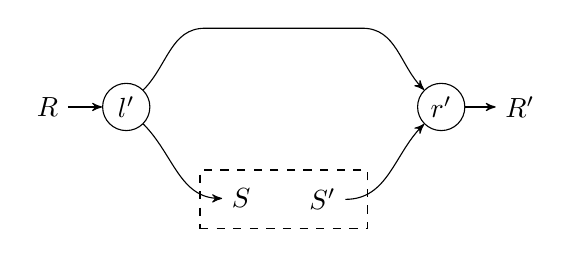
\begin{tikzpicture}
\node[vert] (l) at (0, 0) {$l'$};
\node[vert] (r) at (4, 0) {$r'$};

\node (R) [left of=l] {$R$};
\node (S) [below right = 0.7 and 1 of l] {$S$};
\node (R') [right of=r] {$R'$};
\node (S') [below left = 0.7 and 1 of r] {$S'$};

\draw[->] (R) -- (l);
\draw[->] (l) to[out=south east,in=west] (S);

\draw[<-] (R') -- (r);
\draw[<-] (r) to[out=south west,in=east] (S');

\draw[->] (l) to[out=north east, in=west] ++(1,1)
 to ++(2,0)
 to[out=east, in=north west] (r)
;

\node[draw,dashed,fit=(S) (S'), inner xsep = 8pt] (box) {};
\end{tikzpicture} \\
\raisebox{1.5cm}{$:=$}\qquad
\begin{tikzpicture}
\begin{scope}[on grid]

\node[vert] (l') at (0, 0) {$l'$};
\node[vert, below right = 0.7 and 1 of l'] (l) {$l$};
\node[vert] (r') at (5, 0) {$r'$};
\node[vert, below left = 0.7 and 1 of r'] (r) {$r$};

\node (A) [below right = 0.7 and 1 of l] {$A$};
\node (A') [below left = 0.7 and 1 of r] {$A'$};

\node (R) [left of=l'] {$R$};
\node (R') [right of=r'] {$R'$};

\draw[->] (R) -- (l');
\draw[<-] (R') -- (r');

\draw[->] (l') to[rrel, out=north east, in=west] (1,1)
 to +(3,0)
 to[out=east, in=north west] (r')
;

\draw[->] (l) to[rrel, out=north east, in=west] (1,1)
 to +(1,0)
 to[out=east, in=north west] (r)
;

\draw[->] (l') to[out=south east,in=west] (l);
\draw[->] (r) to[out=east, in=south west] (r');

\draw[->] (l) to[out=south east,in=west] (A);
\draw[<-] (r) to[out=south west,in=east] (A');

\node[draw,dashed,fit=(l) (r), inner xsep = 6pt, inner ysep = 25pt] (box2) {};
\node[draw,dashed,fit=(A) (A'), inner xsep = 8pt] (box) {};
\end{scope}
\end{tikzpicture}
\end{center}

The identity optic $(S, S') \hto (S, S')$ is given by $\langle \lambda^{-1}_S, \lambda_{S'} \rangle$, where $\lambda_S : I \otimes S \to S$ is the left unitor for $S$: 
\begin{center}
\begin{tikzpicture}
\begin{scope}[on grid]
\node[vert] (l) at (0, 0) {$\lambda_S^{-1}$};
\node[vert] (r) at (4, 0) {$\lambda_{S'}$};

\node (S) [left of=l] {$S$};
\node (A) [below right = 0.7 and 1 of l] {$S$};
\node (S') [right of=r] {$S'$};
\node (A') [below left = 0.7 and 1 of r] {$S'$};

\draw[->] (S) -- (l);
\draw[->] (l) to[out=south east,in=west] (A);

\draw[<-] (S') -- (r);
\draw[<-] (r) to[out=south west,in=east] (A');

\draw[->, dotted] (l) to[rrel, out=north east, in=west] (1,1)
 to +(2,0)
 to[out=east, in=north west] (r)
;

\node[draw,dashed,fit=(A) (A'), inner xsep = 8pt] (box) {};
\end{scope}
\end{tikzpicture}
\end{center}
This dashed line above the diagram represents the unit object. As is standard, we will elide the unit object and unitors in future diagrams. The diagram for the identity becomes simply:
\begin{center}
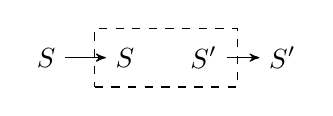
\begin{tikzpicture}
\node (Sin) {$S$};
\node (Sout) [right of=Sin] {$S$};
\node (Spout) [right of=Sout] {$S'$};
\node (Spin) [right of=Spout] {$S'$};

\draw[->] (Sin) -- (Sout);
\draw[->] (Spout) -- (Spin);

\node[draw,dashed,fit=(Sout) (Spout), inner xsep = 4pt] (box) {};
\end{tikzpicture}
\end{center}

\begin{proposition}
The above data form a category $\Optic_\C$.
\end{proposition}
\begin{proof}
In \cite[Section 6]{Doubles} this is proven abstractly, by exhibiting this category as the Kleisli category for a monad in the bicategory $\Prof$. Here we prove the properties directly.

We check associativity of composition equationally. As in the definition of composition, the Fubini theorem for coends allows us to choose representatives for all three optics simultaneously. Suppose we have representatives of three optics $\langle l_1, r_1\rangle : (R, R) \hto (S, S')$ and $\langle l_2, r_2 \rangle : (S, S') \hto (A, A')$ and $\langle l_3, r_3 \rangle : (A, A') \hto (B, B')$, that have complements $M$, $N$ and $P$ respectively. Then:
\begin{align*}
(\langle l_3, r_3 \rangle \circ \langle l_2, r_2 \rangle) \circ \langle l_1, r_1 \rangle 
&= \langle (N \otimes l_3)l_2, r_2(N \otimes r_3) \rangle \circ \langle l_1, r_1 \rangle \\
&= \langle (M \otimes ((N \otimes l_3)l_2))l_1, r_1(M \otimes (r_2(N \otimes r_3))) \rangle \\
&= \langle (M \otimes N \otimes l_3)(M \otimes l_2)l_1, r_1(M \otimes r_2)(M \otimes N \otimes r_3)) \rangle \\
&= \langle l_3, r_3 \rangle \circ (\langle (M \otimes l_2)l_1, r_1(M \otimes r_2) \rangle) \\
&= \langle l_3, r_3 \rangle \circ (\langle l_2, r_2 \rangle \circ \langle l_1, r_1 \rangle)
\end{align*}

For the unit laws, suppose we have $\langle l, r \rangle : (S, S') \hto (A, A')$ with representative $M$. We calculate:
\begin{align*}
\id_{A, A'} \circ \langle l, r\rangle 
&= \langle \lambda^{-1}_A, \lambda_{A'} \rangle \circ \langle l, r\rangle \\
&= \langle (M \otimes \lambda^{-1}_A) l, r (M\otimes  \lambda_{A'})\rangle \\
&= \langle (\lambda^{-1}_M \otimes  A) l, r (\lambda_M \otimes A')\rangle \\
&= \langle l, r (\lambda_M \otimes A') (\lambda^{-1}_M \otimes A')\rangle \\
&= \langle l, r \rangle  \\
\langle l, r \rangle \circ \id_{S, S'} 
&= \langle l, r \rangle \circ \langle \lambda^{-1}_S, \lambda_{S'}\rangle  \\
&= \langle (I \otimes l)\lambda^{-1}_S, \lambda_{S'} (I \otimes r) \rangle \\
&= \langle (\lambda^{-1}_M \otimes S)l, r (\lambda_{M} \otimes S') \rangle \\
&= \langle l, r (\lambda_{M} \otimes S')(\lambda^{-1}_M \otimes S') \rangle \\
&= \langle l, r \rangle
\end{align*}
Where in both cases we have used the naturality of $\lambda$ and coend relations to move $\lambda^{-1}_M$ to the right-hand side of the coend. 
\end{proof}

\begin{remark}
Note that the definition of the $\Optic$ category involves a coend possibly indexed by a large category. To be maximally careful, we should only ever discuss $\Optic$ categories where we know that the coend exists by some other means, e.g., by exhibiting an isomorphism with some other set. For many---but not all---of the examples given later, we provide such an isomorphism.

\todo{How does the doubles paper get away with it?}
\end{remark}

\begin{proposition}
There is a functor $\iota : \C \times \C^\op \to \Optic_\C$, which is given on objects by $\iota(S, S') = (S, S')$ and for a morphism $(f, g) : (S, S') \to (A, A')$ by $\iota(f, g) = \langle \lambda_A^{-1} f, g \lambda_{A'} \rangle$.
\end{proposition}
\begin{proof}
Graphically, this is:
\begin{center}
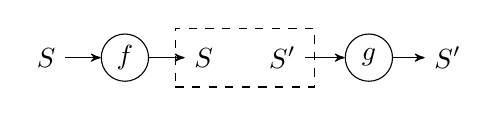
\begin{tikzpicture}
\node (Sin) {$S$};
\node (f) [vert, right of=Sin] {$f$};
\node (Sout) [right of=f] {$S$};
\node (Spout) [right of=Sout] {$S'$};
\node (g) [vert, right = 0.5 of Spout] {$g$};
\node (Spin) [right of=g] {$S'$};

\draw[->] (Sin) -- (f);
\draw[->] (f) -- (Sout);
\draw[->] (Spout) -- (g);
\draw[->] (g) -- (Spin);

\node[draw,dashed,fit=(Sout) (Spout)] (box) {};
\end{tikzpicture}
\end{center}

This preserves identities, as the identity on an object $(S, S')$ in $\Optic_\M$ is defined to be exactly $\langle \lambda^{-1}_S, \lambda_{S'} \rangle$.

To check functoriality, suppose we have $(f, g) : (S, S') \to (A, A')$ and $(f', g') : (A, A') \to (B, B')$ in $\C \times \C^\op$. Then:
\begin{align*}
\iota(f', g') \circ \iota(f, g) 
&= \langle \lambda^{-1}_B f', g' \lambda_{B'} \rangle \circ \langle \lambda^{-1}_A f, g \lambda_{A'} \rangle \\
&= \langle (I\otimes (\lambda^{-1}_B f'))\lambda^{-1}_A f, g \lambda_{A'} (I\otimes (g' \lambda_{B'}))\rangle && \text{(By definition of $\circ$)}\\
&= \langle (I \otimes \lambda^{-1}_B) (I \otimes f')\lambda^{-1}_A f, g \lambda_{A'} (I \otimes g')(I\otimes \lambda_{B'})\rangle && \text{(Functoriality of $I \otimes -$)}\\
&= \langle (I\otimes \lambda^{-1}_B) \lambda^{-1}_B f' f, g g' \lambda_{B'} (I\otimes \lambda_{B'})\rangle && \text{(Naturality of $\lambda$)}\\
&= \langle (\lambda^{-1}_I \otimes B) \lambda^{-1}_B f' f, g g' \lambda_{B'} (\lambda_I \otimes B')\rangle && \text{(Unitality of action)} \\
&= \langle \lambda^{-1}_B f' f, g g' \lambda_{B'} (\lambda_I \otimes B') (\lambda^{-1}_I \otimes B') \rangle && \text{(Coend relation)}  \\
&= \langle \lambda^{-1}_B f'f, g g' \lambda_{B'} \rangle \\
&= \iota(f'f, gg')
\end{align*}
Graphically, there is not much to do:
\begin{center}
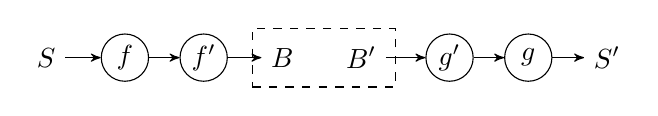
\begin{tikzpicture}
\node (Sin) {$S$};
\node (f) [vert, right of=Sin] {$f$};
\node (f') [vert, right of=f] {$f'$};
\node (Sout) [right of=f'] {$B$};
\node (Spout) [right of=Sout] {$B'$};
\node (g') [vert, right = 0.5 of Spout] {$g'$};
\node (g) [vert, right of=g'] {$g$};
\node (Spin) [right of=g] {$S'$};

\draw[->] (Sin) -- (f);
\draw[->] (f) -- (f');
\draw[->] (f') -- (Sout);
\draw[->] (Spout) -- (g');
\draw[->] (g') -- (g);
\draw[->] (g) -- (Spin);

\node[draw,dashed,fit=(Sout) (Spout)] (box) {};
\end{tikzpicture}
\qquad \raisebox{0.3cm}{$=$} \qquad 
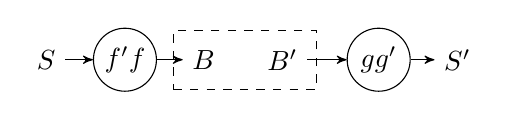
\begin{tikzpicture}
\node (Sin) {$S$};
\node (f) [vertbig, right of=Sin] {$f'f$};
\node (Sout) [right of=f] {$B$};
\node (Spout) [right of=Sout] {$B'$};
\node (g) [vertbig, right = 0.5 of Spout] {$gg'$};
\node (Spin) [right of=g] {$S'$};

\draw[->] (Sin) -- (f);
\draw[->] (f) -- (Sout);
\draw[->] (Spout) -- (g);
\draw[->] (g) -- (Spin);

\node[draw,dashed,fit=(Sout) (Spout)] (box) {};
\end{tikzpicture}
\end{center}

\end{proof}

\begin{remark}
This functor is not necessarily faithful, see Remark \ref{lens-iota-not-faithful}.
\end{remark}

%\todo{This doesn't give us the structure of a `framing', we can only lift vertical arrows to horizontal arrows facing one direction.}

%\begin{theorem}
%$\Optic_\C$ is symmetric monoidal, where $(S, S') \otimes (T, T') = (S \otimes T, S' \otimes T')$, the unit is $(I, I)$, and the action on morphisms induced by
%\begin{align*}
%&\C(S, M \otimes A) \times \C(M \otimes A', S') \times \C(T, N \otimes B) \times \C(N \otimes B', T')\\
%\to \quad&\C(S \otimes T, M \otimes A \otimes N \otimes B) \times \C(M \otimes A' \otimes N \otimes B', S' \otimes T') && \text{(action of $\otimes$ on morphisms in $\C$)}\\
%\to \quad&\C(S \otimes T, M \otimes N \otimes A \otimes B) \times \C(M \otimes N \otimes A' \otimes B', S' \otimes T') && \text{($\otimes$ in $\C$ is symmetric)}\\
%\to \quad&\int^{M \in \C} \C(S \otimes T, M \otimes A \otimes B) \times \C(M \otimes A' \otimes B', S' \otimes T') && \text{(inclusion into coend)}
%\end{align*}
%\end{theorem}
%\begin{proof}
%Equationally, suppose we have representatives $(l, r) : (S \to M \otimes A, M \otimes A' \to S')$ and $(l', r') : (T \to N \otimes B, N \otimes B' \to T')$. Then:
%\begin{align*}
%\langle l, r \rangle \otimes \langle l', r' \rangle &:= \langle (M \otimes s_{A,N} \otimes B)(l \otimes l'), (r \otimes r')(M \otimes s_{A',N} \otimes B') \rangle
%\end{align*}
%This is functorial, as suggested by the equivalence of the following string diagrams:
%\todo{todo}
%%For future convenience, note that 
%%\begin{align*}
%%\langle l, r \rangle \otimes (T, T') &= \langle (M \otimes s_{A,I} \otimes T)(l \otimes \lambda_T), (r \otimes \lambda^{-1}_{T'})(M \otimes s_{A',I}\otimes T') \rangle \\
%%&= \langle (\lambda^{-1}_M \otimes A \otimes T)(M \otimes s_{A,I} \otimes T)(l \otimes \lambda_T), (r \otimes \lambda^{-1}_{T'})(M \otimes s_{A',I}\otimes T')(\lambda_M \otimes A' \otimes T') \rangle \\
%%&= \langle l \otimes T, r \otimes T' \rangle
%%\end{align*}
%%Now we check functoriality. Suppose we have:
%%\begin{align*}
%%\langle l_1, r_1 \rangle : (S_1, S_1') &\hto (S_2, S_2') \\
%%\langle l_2, r_2 \rangle : (S_2, S_2') &\hto (S_3, S_3') \\
%%\langle p_1, q_1 \rangle : (T_1, T_1') &\hto (T_2, T_2') \\
%%\langle p_2, q_2 \rangle : (T_2, T_2') &\hto (T_3, T_3')
%%\end{align*}
%%with complements $M_1, M_2, N_1, N_2$ respectively. Then: \todo {(This is a mess. String diagram?)}
%%\begin{align*}
%%&(\langle l_2, r_2 \rangle \otimes \langle p_2, q_2 \rangle) \circ (\langle l_1, r_1 \rangle \otimes \langle p_1, q_1 \rangle) \\
%%= \; &\langle (M_2 \otimes s_{S_3,N_2} \otimes T_3)(l_2 \otimes p_2), (r_2 \otimes q_2)(M_2 \otimes s_{S_3',N_2} \otimes T_3') \rangle \\
%%&\circ \langle (M_1 \otimes s_{S_2,N_1} \otimes T_2)(l_1 \otimes p_1), (r_1 \otimes q_1)(M_1 \otimes s_{S_2',N_1} \otimes T_2') \rangle \\
%%= \; & \langle (M_1 \otimes N_1 \otimes M_2 \otimes s_{S_3,N_2} \otimes T_3)(M_1 \otimes N_1 \otimes l_2 \otimes p_2)(M_1 \otimes s_{S_2,N_1} \otimes T_2)(l_1 \otimes p_1), \\
%%&\;(r_1 \otimes q_1)(M_1 \otimes s_{S_2',N_1} \otimes T_2')(M_1 \otimes N_1 \otimes r_2 \otimes q_2)(M_1 \otimes N_1 \otimes M_2 \otimes s_{S_3',N_2} \otimes T_3') \rangle \\
%%= \; & \langle (M_1 \otimes N_1 \otimes M_2 \otimes s_{S_3,N_2} \otimes T_3)(M_1 \otimes s_{(M_2 \otimes S_3),N_1} \otimes T_3)(M_1 \otimes  l_2 \otimes N_1 \otimes p_2)(l_1 \otimes p_1), \\
%%&\;(r_1 \otimes q_1)(M_1 \otimes r_2 \otimes N_1 \otimes q_2)(M_1 \otimes s_{(M_2 \otimes S_3'),N_1} \otimes T_3')(M_1 \otimes N_1 \otimes M_2 \otimes s_{S_3',N_2} \otimes T_3') \rangle \\
%%= \; & \langle (M_1 \otimes N_1 \otimes M_2 \otimes s_{S_3,N_2} \otimes T_3)(M_1 \otimes s_{(M_2 \otimes S_3),N_1} \otimes T_3)((M_1 \otimes l_2)l_1\otimes (N_1 \otimes p_2)p_1), \\
%%&\;(r_1(M_1 \otimes r_2) \otimes q_1(N_1 \otimes q_2))(M_1 \otimes s_{(M_2 \otimes S_3'),N_1} \otimes T_3')(M_1 \otimes N_1 \otimes M_2 \otimes s_{S_3',N_2} \otimes T_3') \rangle \\
%%= \; & \text{\todo{(Add a $s_{M_2, N_1}$ to either side of the coend, then appeal to coherence)}} \\
%%= \; &\langle (M_1 \otimes M_2 \otimes s_{(N_1 \otimes N_2),S_3} \otimes T_3)((M_1 \otimes l_2)l_1\otimes (N_1 \otimes p_2)p_1) ,  \\
%%&\;(r_1(M_1 \otimes r_2) \otimes q_1(N_1 \otimes q_2))(M_1 \otimes M_2 \otimes s_{(N_1 \otimes N_2),S'_3} \otimes T'_3) \rangle \\
%%= \; &\langle (M_1 \otimes l_2)l_1, r_1(M_1 \otimes r_2) \rangle \otimes \langle (N_1 \otimes p_2)p_1, q_1(N_1 \otimes q_2) \rangle \\
%%= \; &(\langle l_2, r_2 \rangle  \circ \langle l_1, r_1 \rangle) \otimes (\langle p_2, q_2 \rangle \circ \langle p_1, q_1 \rangle)
%%\end{align*}
%
%The structure morphisms are all lifted from the structure morphisms in $\C$:
%\begin{align*}
%\alpha_{(R, R'), (S, S'), (T, T')} &:= \iota(\alpha_{R,S,T}, \alpha_{R',S',T'}^{-1}) \\
%\lambda_{(S, S')} &:= \iota(\lambda_{(S, S')}, \lambda_{(S, S')}^{-1}) \\
%\rho_{(S, S')} &:= (\rho_{(S, S')}, \rho_{(S, S')}^{-1}) \\
%s_{(S, S'), (T, T')} &:= \iota(s_{S, T}, s_{T', S'})
%\end{align*}
% 
%Note that because $\iota(S, S') = (S, S')$, required equations for $\iota$ to be a monoidal functor hold by definition (although we don't yet know that $\Optic_\otimes$ is monoidal). The pentagon and triangle axioms then hold in $\Optic_\otimes$, as they are the image of the same axioms in $\C \times \C^\op$ under $\iota$. The only remaining thing to verify is that these structure maps are natural in $\Optic_\otimes$. 
%
%Let us check that $\alpha_{(R, R'), (S, S'), (T, T')}$ is natural in $(R, R')$. Suppose $f : (Q, Q') \hto (R, R')$ has representative $(l, r) : (Q \to M \otimes R, M \otimes R' \to Q')$, then:
%\begin{align*}
%&\alpha_{(R, R'), (S, S'), (T, T')} \circ (f \otimes (S, S')) \otimes (T, T') \\
%&= \iota(\alpha_{R,S,T}, \alpha_{R',S',T'}^{-1})  \circ (\langle l, r \rangle \otimes (S, S')) \otimes (T, T') \\
%&= \langle\lambda_{R \otimes (S \otimes T)}\alpha_{R,S,T}, \alpha_{R',S',T'}^{-1} \lambda^{-1}_{(R' \otimes S') \otimes T'} \rangle  \circ \left\langle (l \otimes S) \otimes T, (r \otimes S') \otimes T' \right\rangle \\
%&=\left\langle (M \otimes \lambda_{R \otimes (S \otimes T)}\alpha_{R,S,T})((l \otimes S) \otimes T), ((r \otimes S') \otimes T') (M \otimes \alpha_{R',S',T'}^{-1} \lambda^{-1}_{(R' \otimes S') \otimes T'} ) \right\rangle \\
%&=\left\langle (M \otimes \alpha_{R,S,T})((l \otimes S) \otimes T), ((r \otimes S') \otimes T') (M \otimes \alpha_{R',S',T'}^{-1} )\right\rangle \\
%&=\left\langle (l \otimes (S \otimes T))\alpha_{Q,S,T}, \alpha_{Q',S',T'}^{-1}(r \otimes (S' \otimes T')) \right\rangle \\
%&= \langle (I \otimes l \otimes (S \otimes T)) \lambda_{Q \otimes (S \otimes T)}\alpha_{Q,S,T}, (I \times r \otimes (S' \otimes T')) \alpha_{Q',S',T'}^{-1} \lambda^{-1}_{Q' \otimes (S' \otimes T')}\rangle \\
%&= \langle l \otimes (S \otimes T), r \otimes (S' \otimes T')\rangle \circ \left\langle \lambda_{Q \otimes (S \otimes T)}\alpha_{Q,S,T}, \alpha_{Q',S',T'}^{-1} \lambda^{-1}_{Q' \otimes (S' \otimes T')} \right\rangle \\
%&= \langle l, r \rangle \otimes ((S, S') \otimes (T, T')) \circ \iota(\alpha_{Q,S,T}, \alpha_{Q',S',T'}^{-1}) \\
%&= f \otimes ((S, S') \otimes (T, T')) \circ \alpha_{(Q, Q'), (S, S'), (T, T')} 
%\end{align*}
%\todo{There is some cheating going on here, composition actually adds an extra $\alpha$, but that wouldn't get in the way.}
%\end{proof}

\begin{theorem}
$\Optic_\C$ is symmetric monoidal, where $(S, S') \otimes (T, T') = (S \otimes T, S' \otimes T')$, the unit is $(I, I)$, and the action on morphisms is given by:
\begin{center}
\begin{tikzpicture}
\begin{scope}[on grid]

\node[vert] (l) at (0, 0) {$l$};
\node[vert] (r) at (6, 0) {$r$};

\node (S) [left of=l] {$S$};
\node (A) [below right = 2 and 2 of l] {$A$};
\node (S') [right of=r] {$S'$};
\node (A') [below left = 2 and 2 of r] {$A'$};

\draw[->] (S) -- (l);
\draw[->] (l) to[out=south east,in=west] (A);

\draw[<-] (S') -- (r);
\draw[<-] (r) to[out=south west,in=east] (A');

\draw[->] (l) to[rrel, out=north east, in=west] (1,1)
 to ++(4,0)
 to[out=east, in=north west] (r)
;

\node[vert] (l') at (0, -2) {$l'$};
\node[vert] (r') at (6, -2) {$r'$};

\node (T) [left of=l'] {$T$};
\node (B) [below right = 1 and 2 of l'] {$B$};
\node (T') [right of=r'] {$T'$};
\node (B') [below left = 1 and 2 of r'] {$B'$};

\draw[->] (T) -- (l');
\draw[->] (l') to[out=south east,in=west] (B);

\draw[<-] (T') -- (r');
\draw[<-] (r') to[out=south west,in=east] (B');

\draw[->] (l') 
 to[rrel, out=north east, in=west] (2,2)
 to ++(2,0)
 to[out=east, in=north west] (r')
;

\node[draw,dashed,fit=(A) (A') (B) (B'), inner xsep = 8pt] (box) {};

\end{scope}
\end{tikzpicture}
\end{center}
\end{theorem}
\begin{proof}
Equationally, suppose we have optics $S \hto A$ and $T \hto B$ with representatives:
\begin{align*}
(l, r) &: (S \to M \otimes A, M \otimes A' \to S') \\
(l', r') &: (T \to N \otimes B, N \otimes B' \to T')
\end{align*}
Then:
\begin{align*}
\langle l, r \rangle \otimes \langle l', r' \rangle &:= \langle (M \otimes s_{A,N} \otimes B)(l \otimes l'), (r \otimes r')(M \otimes s_{A',N} \otimes B') \rangle
\end{align*}
This is functorial, as suggested by the equivalence of the following string diagrams:
\todo{todo}
%For future convenience, note that 
%\begin{align*}
%\langle l, r \rangle \otimes (T, T') &= \langle (M \otimes s_{A,I} \otimes T)(l \otimes \lambda_T), (r \otimes \lambda^{-1}_{T'})(M \otimes s_{A',I}\otimes T') \rangle \\
%&= \langle (\lambda^{-1}_M \otimes A \otimes T)(M \otimes s_{A,I} \otimes T)(l \otimes \lambda_T), (r \otimes \lambda^{-1}_{T'})(M \otimes s_{A',I}\otimes T')(\lambda_M \otimes A' \otimes T') \rangle \\
%&= \langle l \otimes T, r \otimes T' \rangle
%\end{align*}
%Now we check functoriality. Suppose we have:
%\begin{align*}
%\langle l_1, r_1 \rangle : (S_1, S_1') &\hto (S_2, S_2') \\
%\langle l_2, r_2 \rangle : (S_2, S_2') &\hto (S_3, S_3') \\
%\langle p_1, q_1 \rangle : (T_1, T_1') &\hto (T_2, T_2') \\
%\langle p_2, q_2 \rangle : (T_2, T_2') &\hto (T_3, T_3')
%\end{align*}
%with complements $M_1, M_2, N_1, N_2$ respectively. Then: \todo {(This is a mess. String diagram?)}
%\begin{align*}
%&(\langle l_2, r_2 \rangle \otimes \langle p_2, q_2 \rangle) \circ (\langle l_1, r_1 \rangle \otimes \langle p_1, q_1 \rangle) \\
%= \; &\langle (M_2 \otimes s_{S_3,N_2} \otimes T_3)(l_2 \otimes p_2), (r_2 \otimes q_2)(M_2 \otimes s_{S_3',N_2} \otimes T_3') \rangle \\
%&\circ \langle (M_1 \otimes s_{S_2,N_1} \otimes T_2)(l_1 \otimes p_1), (r_1 \otimes q_1)(M_1 \otimes s_{S_2',N_1} \otimes T_2') \rangle \\
%= \; & \langle (M_1 \otimes N_1 \otimes M_2 \otimes s_{S_3,N_2} \otimes T_3)(M_1 \otimes N_1 \otimes l_2 \otimes p_2)(M_1 \otimes s_{S_2,N_1} \otimes T_2)(l_1 \otimes p_1), \\
%&\;(r_1 \otimes q_1)(M_1 \otimes s_{S_2',N_1} \otimes T_2')(M_1 \otimes N_1 \otimes r_2 \otimes q_2)(M_1 \otimes N_1 \otimes M_2 \otimes s_{S_3',N_2} \otimes T_3') \rangle \\
%= \; & \langle (M_1 \otimes N_1 \otimes M_2 \otimes s_{S_3,N_2} \otimes T_3)(M_1 \otimes s_{(M_2 \otimes S_3),N_1} \otimes T_3)(M_1 \otimes  l_2 \otimes N_1 \otimes p_2)(l_1 \otimes p_1), \\
%&\;(r_1 \otimes q_1)(M_1 \otimes r_2 \otimes N_1 \otimes q_2)(M_1 \otimes s_{(M_2 \otimes S_3'),N_1} \otimes T_3')(M_1 \otimes N_1 \otimes M_2 \otimes s_{S_3',N_2} \otimes T_3') \rangle \\
%= \; & \langle (M_1 \otimes N_1 \otimes M_2 \otimes s_{S_3,N_2} \otimes T_3)(M_1 \otimes s_{(M_2 \otimes S_3),N_1} \otimes T_3)((M_1 \otimes l_2)l_1\otimes (N_1 \otimes p_2)p_1), \\
%&\;(r_1(M_1 \otimes r_2) \otimes q_1(N_1 \otimes q_2))(M_1 \otimes s_{(M_2 \otimes S_3'),N_1} \otimes T_3')(M_1 \otimes N_1 \otimes M_2 \otimes s_{S_3',N_2} \otimes T_3') \rangle \\
%= \; & \text{\todo{(Add a $s_{M_2, N_1}$ to either side of the coend, then appeal to coherence)}} \\
%= \; &\langle (M_1 \otimes M_2 \otimes s_{(N_1 \otimes N_2),S_3} \otimes T_3)((M_1 \otimes l_2)l_1\otimes (N_1 \otimes p_2)p_1) ,  \\
%&\;(r_1(M_1 \otimes r_2) \otimes q_1(N_1 \otimes q_2))(M_1 \otimes M_2 \otimes s_{(N_1 \otimes N_2),S'_3} \otimes T'_3) \rangle \\
%= \; &\langle (M_1 \otimes l_2)l_1, r_1(M_1 \otimes r_2) \rangle \otimes \langle (N_1 \otimes p_2)p_1, q_1(N_1 \otimes q_2) \rangle \\
%= \; &(\langle l_2, r_2 \rangle  \circ \langle l_1, r_1 \rangle) \otimes (\langle p_2, q_2 \rangle \circ \langle p_1, q_1 \rangle)
%\end{align*}

The structure morphisms are all lifted from the structure morphisms in $\C$:
\begin{align*}
\alpha_{(R, R'), (S, S'), (T, T')} &:= \iota(\alpha_{R,S,T}, \alpha_{R',S',T'}^{-1}) \\
\lambda_{(S, S')} &:= \iota(\lambda_{(S, S')}, \lambda_{(S, S')}^{-1}) \\
\rho_{(S, S')} &:= \iota(\rho_{(S, S')}, \rho_{(S, S')}^{-1}) \\
s_{(S, S'), (T, T')} &:= \iota(s_{S, T}, s_{T', S'})
\end{align*}
 
Note that because $\iota(S, S') = (S, S')$, required equations for $\iota$ to be a monoidal functor hold by definition (although we don't yet know that $\Optic_\otimes$ is monoidal). The pentagon and triangle axioms then hold in $\Optic_\otimes$, as they are the image of the same axioms in $\C \times \C^\op$ under $\iota$. The only remaining thing to verify is that these structure maps are natural in $\Optic_\otimes$. 

Let us check that $\alpha_{(R, R'), (S, S'), (T, T')}$ is natural in $(R, R')$. Suppose $f : (Q, Q') \hto (R, R')$ has representative $(l, r) : (Q \to M \otimes R, M \otimes R' \to Q')$, then:
\begin{align*}
&\alpha_{(R, R'), (S, S'), (T, T')} \circ (f \otimes (S, S')) \otimes (T, T') \\
&= \iota(\alpha_{R,S,T}, \alpha_{R',S',T'}^{-1})  \circ (\langle l, r \rangle \otimes (S, S')) \otimes (T, T') \\
&= \langle\lambda_{R \otimes (S \otimes T)}\alpha_{R,S,T}, \alpha_{R',S',T'}^{-1} \lambda^{-1}_{(R' \otimes S') \otimes T'} \rangle  \circ \left\langle (l \otimes S) \otimes T, (r \otimes S') \otimes T' \right\rangle \\
&=\left\langle (M \otimes \lambda_{R \otimes (S \otimes T)}\alpha_{R,S,T})((l \otimes S) \otimes T), ((r \otimes S') \otimes T') (M \otimes \alpha_{R',S',T'}^{-1} \lambda^{-1}_{(R' \otimes S') \otimes T'} ) \right\rangle \\
&=\left\langle (M \otimes \alpha_{R,S,T})((l \otimes S) \otimes T), ((r \otimes S') \otimes T') (M \otimes \alpha_{R',S',T'}^{-1} )\right\rangle \\
&=\left\langle (l \otimes (S \otimes T))\alpha_{Q,S,T}, \alpha_{Q',S',T'}^{-1}(r \otimes (S' \otimes T')) \right\rangle \\
&= \langle (I \otimes l \otimes (S \otimes T)) \lambda_{Q \otimes (S \otimes T)}\alpha_{Q,S,T}, (I \times r \otimes (S' \otimes T')) \alpha_{Q',S',T'}^{-1} \lambda^{-1}_{Q' \otimes (S' \otimes T')}\rangle \\
&= \langle l \otimes (S \otimes T), r \otimes (S' \otimes T')\rangle \circ \left\langle \lambda_{Q \otimes (S \otimes T)}\alpha_{Q,S,T}, \alpha_{Q',S',T'}^{-1} \lambda^{-1}_{Q' \otimes (S' \otimes T')} \right\rangle \\
&= \langle l, r \rangle \otimes ((S, S') \otimes (T, T')) \circ \iota(\alpha_{Q,S,T}, \alpha_{Q',S',T'}^{-1}) \\
&= f \otimes ((S, S') \otimes (T, T')) \circ \alpha_{(Q, Q'), (S, S'), (T, T')} 
\end{align*}
\todo{There is some cheating going on here, composition actually adds an extra $\alpha$, but that wouldn't get in the way.}
\end{proof}

\begin{remark}
In the Haskell \texttt{lens} library, the monoidal product on optics is denoted ``\texttt{alongside}'' for the product and ``\texttt{without}'' for the coproduct.
\end{remark}

\begin{proposition}
If $\C$ is a strict symmetric monoidal category then $\Optic_\C$ is also strict.
\end{proposition}
\begin{proof}
The structure maps of $\Optic_\C$ are given by $\iota$ applied to the structure maps of $\C$. If the latter are identities, then so are the former---the identity morphisms in $\Optic_\C$ are by definition $\iota(\id_S, \id_S')$.
\end{proof}

\begin{proposition}
$\iota : \C \times \C^\op \to \Optic_\C$ is a strong monoidal functor. 
\end{proposition}
\begin{proposition}
\todo{todo}
\end{proposition}

%\begin{proposition}
%Any isomorphism $p : (S, S') \hto (A, A')$ in $\Optic_\C$ is of the form $\iota(f, g)$ for two isomorphisms $S \to A$ and $A' \to S'$ in $\C$.
%\end{proposition}
%\begin{proof}
%\todo{This might not actually be true..}
%\end{proof}

There is some further useful structure in $\Optic_\C$. 
\begin{proposition}
\label{prop-costates}
The set of costates $(S, S') \hto (I, I)$ is isomorphic to $\C(S, S')$.
\end{proposition}
\begin{proof}
\begin{align*}
\Optic_\C((S, S'), (I, I)) 
&= \int^{M \in \C} \C(S, M \otimes I) \times \C(M \otimes I, S') \\
&\cong \int^{M \in \C} \C(S, M) \times \C(M, S') \\
&\cong \C(S, S')
\end{align*}
\end{proof}

\todo{Is there a relationship between $\Optic_\C/(I, I)$ and $[2, \C]$?}

In particular, for any $M \in \C$, the image of the identity yields an optic $c_M : (M, M) \hto (I, I)$, that we will call the connector.

States are not as easy to describe in general, however:

\begin{proposition}
Suppose the monoidal unit $I$ of $\C$ is terminal. Then the set of states $(I, I) \hto (A, A')$ is isomorphic to $\C(I, A)$.
\end{proposition}
\begin{proof}
First, note that
\begin{align*}
\Optic_\C((I,I), (A,A')) 
&= \int^{M \in \C} \C(I, M \otimes A) \times \C(M \otimes A', I) \\
&\cong \int^{M \in \C} \C(I, M \otimes A).
\end{align*}
Because the interior of this coend is mute in the contravariant position, the coend is equal to the colimit of the functor $\C(I, - \otimes A) : \C \to \Set$. But $\C$ has a terminal object, so $\int^{M \in \C} \C(I, M \otimes A) \cong \C(I, I \otimes A) \cong \C(I, A)$.
\end{proof}

\begin{proposition}
\todo{Entrywise Coproduct}
\end{proposition}

\begin{remark}
The motivating example here is that of coproducts distributing over the tensor product.
\end{remark}

\begin{proposition}
A monoidal functor $F : \C \to \D$ induces a  functor $\Optic(F) : \Optic_\C \to \Optic_\D$
\end{proposition}
\begin{proof}
On objects this is simply $\Optic(F)(S, S') = (FS, FS')$. On a morphism $\langle l, r \rangle : (S, S') \to (A, A')$, we define
\begin{align*}
F\langle l, r \rangle := \langle \phi^{-1}_{M,A} (Fl), (Fr) \phi_{M,A'}\rangle
\end{align*}
where $\phi_{M,A} : FM \otimes FA \to F(M \otimes A)$ is the structure map of the monoidal functor.
\todo{functoriality}
\todo{monoidality}
\end{proof}

\begin{proposition}
Together this operation defines a \todo{pseudo?}functor $\Optic : \SymmMonCat \to \SymmMonCat$.
\end{proposition}
\begin{proof}
\todo{todo}
\end{proof}

\subsection{Teleological Categories}
\label{teleological-categories}

Categories of optics admit their own diagrammatic language, by virtue of them being \emph{teleological categories}. In fact, we show in Theorem \ref{optic-is-free-teleological-cat} that $\Optic_\C$ is the free teleological category on a collection of dualisable morphisms $\C$.

In this section we assume that $\C$ is a \emph{strict} symmetric monoidal category.

\begin{definition}[{\cite[Definition 5.1]{CoherenceForLenses}}]
A \emph{teleological category is} a symmetric monoidal category $(\C, \otimes, I)$, equipped with:
\begin{itemize}
\item A wide symmetric monoidal subcategory $\C_d$ of \emph{dualisable morphisms}, with an involutive strong symmetric monoidal functor $(-)^* : \C_d \to \C_d^\op$; and,
\item A family of morphisms $\varepsilon_X : X \otimes X^* \to I$, called \emph{counits}, natural with respect to the morphisms in $\C_d$, such that
\[
\begin{tikzcd}
X \otimes Y^* \ar[r, "f \otimes Y^*"]  \ar[d, "X \otimes f^*", swap] & Y \otimes Y^* \ar[d, "\varepsilon_Y"] \\
X \otimes X^* \ar[r, "\varepsilon_X", swap] & I
\end{tikzcd} \hspace{1cm}
\begin{tikzcd}
X^* \otimes X \ar[r, "s_{X^*, X}"]  \ar[dr, "\varepsilon_{X^*}", swap] & X \otimes X^* \ar[d, "\varepsilon_X"] \\
& I
\end{tikzcd} \hspace{1cm}
\begin{tikzcd}
X \otimes Y \otimes X^* \otimes Y^* \ar[r, "X \otimes s_{Y,X^*} \otimes X^*"]  \ar[dr, "\varepsilon_{X \otimes Y}", swap] & X \otimes X^* \otimes Y \otimes Y^* \ar[d, "\varepsilon_X \otimes \varepsilon_Y"] \\
& I
\end{tikzcd}
\]
commute for all $f : X \to Y$ is in $\C_d$.
\end{itemize}
\end{definition}
Note that because $\C_d$ is symmetric monoidal and has the same collection of objects as $\C$, the symmetric monoidal structure of $\C$ must all be contained in $\C_d$.

\begin{example}
Any symmetric monoidal category with terminal monoidal unit is trivially teleological, setting the dualisable morphisms to be only the structure maps of the monoidal category.
\end{example}

\todo{\begin{example}
The funny graph example from the coherence paper?
\end{example}}

\begin{remark}
Compact closed categories very nearly form an example of teleological categories. In a compact closed category, there are canonical isomorphisms $(X \otimes Y)^* \cong Y^* \otimes X^*$. In a teleological category, however, duality does not reverse the order of the tensor. \todo{If $\C$ is strict though, does this matter?}
\end{remark}

\begin{definition}
A \emph{teleological functor} $F : \C \to \D$ is a strong symmetric monoidal functor that restricts to a functor $F_d : \C_d \to \D_d$ on the dualisable subcategories, and such that $F(\varepsilon_X) = \varepsilon_{FX}$ \todo{up to the structure isomorphisms of $F$...}
\end{definition}

Together we have $\Tele$, the (1-)category of teleological categories and functors. There are evident functors $U : \Tele \to \SymmMonCat$ and $(-)_d : \Tele \to \SymmMonCat$, that take a teleological category to its underlying symmetric monoidal category and subcategory of dualisable morphisms respectively.

\begin{proposition}
$\Optic_\C$ forms a teleological category, where:
\begin{itemize}
\item The dualisable morphisms are all morphisms of the form $\iota(f, g)$;
\item The involution is given on objects by $(S, S')^* = (S', S)$, and on a morphism $\iota(f, g)$ by $\iota(g, f)$;
\item The counit $\varepsilon_{(S, S')}$  is given by the connector $c_{S \otimes S'}$.
\end{itemize}
\end{proposition}
\begin{proof}
That morphisms of the form $\iota(f, g)$ constitute a category and that $(-)^*$ is a symmetric monoidal involution is clear. \todo{actually check monoidal part}

To check extranaturality, suppose we have a dualisable optic $\iota(f, g) : (X, X') \to (Y, Y')$, so $f : X \to Y$ and $g : Y' \to X'$. Extranaturality is witnessed by the equality of the string diagrams:
\begin{center}
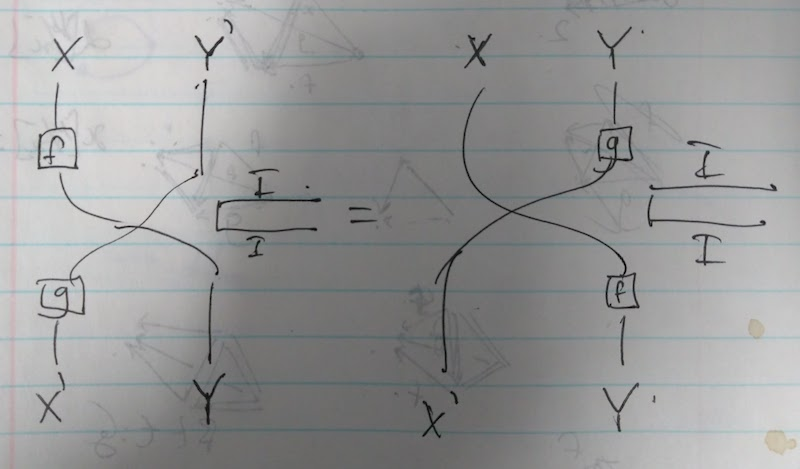
\includegraphics[width=.4\textwidth]{diagrams/counit-extranaturality}
\end{center}
Symmetry:
\begin{center}
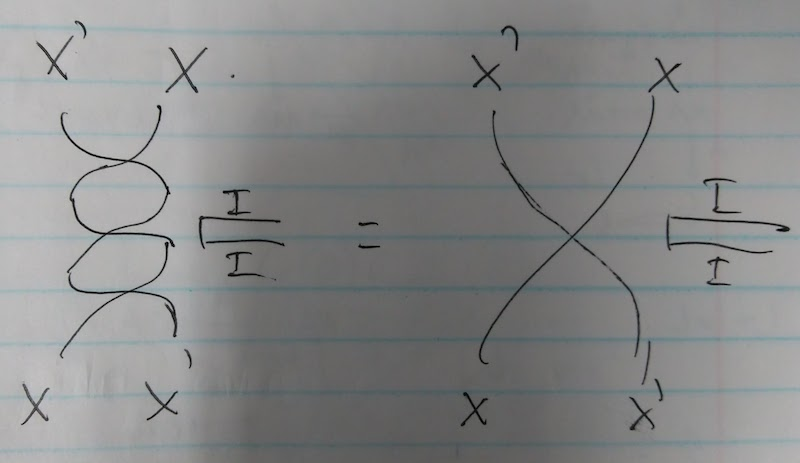
\includegraphics[width=.4\textwidth]{diagrams/counit-symmetry}
\end{center}
Monoidal:
\begin{center}
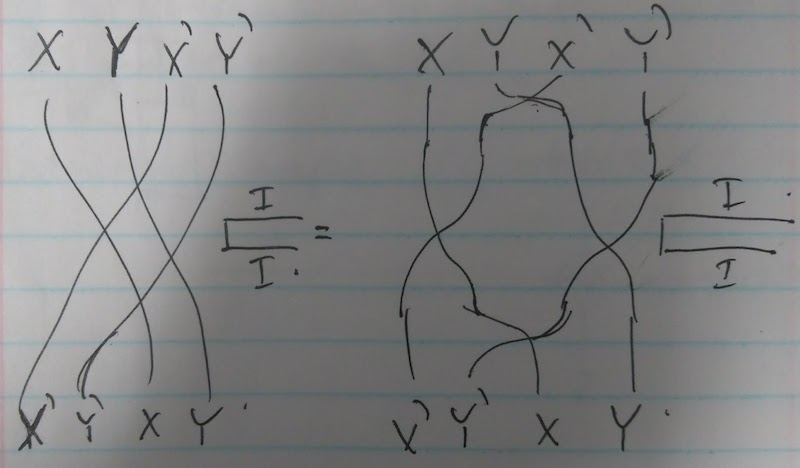
\includegraphics[width=.4\textwidth]{diagrams/counit-monoidal}
\end{center}

Note that the diagrams required to commute all terminate with the unit $I$, so in view of Proposition \ref{prop-costates} we should not be surprised that they correspond to equality of maps in $\C$.
\end{proof}

\todo{They stress about the empty set, have I avoided that issue?}

\begin{proposition}
$\Optic : \SymmMonCat \to \Tele$ is a functor.
\end{proposition}
\begin{proof}
We have to show that for a symmetric monoidal functor $F : \C \to \D$, the induced functor $\Optic_\C \to \Optic_\D$ is teleological.

\todo{todo}
\end{proof}

\begin{proposition}
\label{prop-optic-decompose}
Suppose $p : (S, S') \to (A, A')$ has representative $\langle l, r \rangle$. Then 
\begin{align*}
p = (\varepsilon_{(M, I)} \otimes (A, A'))\iota(l, r).
\end{align*}
\end{proposition}
\begin{proof}
\todo{by string diagram}
\end{proof}

\begin{theorem}
\label{optic-is-free-teleological-cat}
Suppose $\C$ is a \todo{strict} symmetric monoidal category and $\T$ is a teleological category. For all monoidal functors $F : \C \to \T_d$, there exists a teleological functor $K : \Lens_\C \to \T$, unique up to isomorphism, such that $Kj \cong F$.
%$\Optic$ is left adjoint to $(-)_d$, so $\Optic_\C$ is the free teleological category on a category of dualisable morphisms $\C$.
\end{theorem}
\begin{proof}
\todo{This is the point at which I have run in to trouble: TODO}

%On objects, define $K(S, S') = FS \otimes (FS')*$. Suppose $p : (S, S') \hto (A, A')$ is an optic with representative $\langle l, r \rangle$. By Proposition \ref{prop-optic-decompose} and the previous Lemma, $p$ may be decomposed as:
%\begin{align*}
%\langle l, r \rangle = (\varepsilon_{(M, I)}\iota(\rho_M^{-1}, \lambda_M) \otimes \id_{(A, A')})\iota(l, s_{M,A'}r)
%\end{align*}
%But now, in order for $K$ to be a teleological functor with $Kj \cong F$, each piece of this expression must be preserved by $K$, so we define:
%\begin{align*}
%K\langle l, r \rangle = (\varepsilon_{FM} \otimes \id_{FA \otimes FA'})(Fl \otimes s_{FM,FA'} (Fr)^* )
%\end{align*}
%
%This is much easier to understand in the diagrammatic language for teleological categories: \todo{todo}
%
%We now have to check that this is well defined. \todo{todo}
%
%\todo{incomplete}
\end{proof}

\begin{remark}
It is unclear whether an argument like this can work in the case $\C$ is \emph{not} strict. There are a number of issues:

\begin{itemize}
\item Given $f : S \to A$ and $g : A' \to S'$, the optic $j(f) \otimes j(g)^* : (S \otimes I, I \otimes S') \hto (A \otimes I, I \otimes A')$ is not equal to $\iota(f, g)$. It is also not in a form that can be composed with the unitors of $\Optic_\C$, as the $I$s are not all on the same side.
\item \todo{wasn't there more?}
\end{itemize}

One possible workaround: We could extend the category of optics so it contains the image of $\C$ and its duals directly, without needing ghost morphisms $I \to I$ to face the other direction. So there are also objects $(S)$, and a morphism $(S) \hto (A)$ is either an $f : S \to A$ or the formal dual of a $g : A \to S$, and a morphism $(S) \hto (A, A')$ is an optic $(S, I) \hto (A, A')$. 

There are several cases involved when composing morphisms and tensoring objects, depending on which kinds of objects are involved. This is significantly fiddlier, but it should allow a version of Proposition \ref{prop-optic-decompose} to apply to any $\C$.
\end{remark}

\subsection{Optics for a Monoidal Action}

To capture the \texttt{Iso}s, \texttt{Traversal}s and \texttt{Setter}s of the Haskell \texttt{lens} library (see \ref{lawful-examples}), we generalise to the case of a monoidal action of one category on another.

\begin{definition}
Let $\C$ be a category and $(\M, \otimes, I)$ a monoidal category. An \emph{action of $\M$ on $\C$} is a strong monoidal functor $a : \M \to [\C, \C]$. The action of an object $M \in \M$ on $A \in \C$ is written $MA$.
\end{definition}

Given such an action, we define 
\begin{align*}
\Optic_\M((S, S'), (A, A')) := \int^{M \in \C} \C(S, MA) \times \C(MA', S')
\end{align*}

\begin{proposition}
We have a category $\Optic_\M$ and a functor $\iota : \C \times \C^\op \to \Optic_\M$. \qed
\end{proposition}

For the remainder of the paper we work in this slightly more general setting.

\section{Lawful Optics}
\todo{intro}

\begin{remark}
In this section we will focus only on optics of the form $p : (S,S) \hto (A, A)$. We therefore abbreviate $\Optic_\M((S, S), (A, A))$ as $\Optic_\M(S, A)$ and $p : (S, S) \hto (A, A)$ as $p : S \hto A$.
\end{remark}

For a fixed $M \in \M$, there is a map $\C(S, M A) \times \C(M A, S) \to \C(S, S)$ given by composition. This induces a map $outside : \Optic_\M(S, A) \to \C(S, S)$. By composition in the other direction we have a map $\C(S, M A) \times \C(M A, S) \to \C(M A, M A)$. Including this object $\C(M A, M A)$ into the coend $\int^{M \in \M} \C(M A, M A)$, we induce a map $inside : \Optic_\M(S, A) \to \int^{M \in \M} \C(M A, M A)$. 
\begin{definition}
An optic $p : S \hto A$ is \emph{lawful} if $outside(p) = \id_S$, and $inside(p) = \langle t A \rangle$ for some $t : M \to M$ in $\M$.
\end{definition}

\begin{proposition}
There is an subcategory $\Lawful_\M$ of $\Optic_\M$ given by objects of the form $(X, X)$ and lawful optics between them.
\end{proposition}
\begin{proof}
The identity optic $\iota(\id_X, \id_X)$ is clearly lawful.

Suppose we have two lawful optics $\langle l, r \rangle : R \hto S$ and $\langle l', r' \rangle : S \hto A$, where $l : R \to MS$ and $l' : S \to NA$, and such that $lr = \phi S$ and $l'r' = \psi A$. Then the composite $\langle (Ml')l, r (Mr')  \rangle$ is also a lawful optic:
\begin{align*}
r (Mr')(Ml')l &= r M(r'l') l = rl = \id_S
\intertext{and}
(Ml')l r (Mr') &= (Ml')(\phi S)(Mr') \\ 
&= (\phi NA) M(l')M(r') \\ 
&= (\phi NA) M(l'r') \\
&= (\phi NA) M(\psi A) \\
&= \phi(\psi A)
\end{align*}
by the naturality of the action of $\M$.
\end{proof}

\begin{proposition}
\label{prop-onthenose}
If $p : S \to A$ is a lawful optic, then there exists a representative $p = \langle l, r \rangle$ such that $rl = \phi A$ on the nose for some $\phi : M \to M$.
\end{proposition}
\begin{proof}
\todo{This is painful but seems important. There may be a more general principle at work here but I couldn't see it. Put in an appendix?}

There is a well known formula for the coend as the coequaliser in the diagram
\[
\begin{tikzcd}
\coprod_{M \to N} P(N, M) \ar[r,shift left=.75ex]  \ar[r,shift right=.75ex] & \coprod_{M \in \M} P(M, M) \ar[r] & \int^{M \in \M} P(M, M)
\end{tikzcd}
\]
where $P$ is a functor $\M^\op \times \M \to \E$.

In our case $\E = \Set$, and unwinding the coequaliser this states that $\int^{M \in \M} \C(M A, M A)$ is a quotient of the set $\coprod_{M \in \M} \C(M A, M A)$. Two morphisms $f : M A \to M A$ and $g : N A \to N A$ are identified when there exists a $k : N A \to M A$ and natural transformation $\phi : M \to N$ such that the diagram
\[
\begin{tikzcd}
M A \ar[r, "\phi_A"] \ar[d, "f", swap] & N A \ar[d, "g"] \ar[dl, "k"] \\
M A \ar[r, "\phi_A", swap] & N A
\end{tikzcd}
\]
commutes. This gives a binary relation $f \rightsquigarrow g$ that is not likely to be symmetric or transitive. The coend is obtained by identifying all morphisms related in this way, so in all, $\langle f \rangle = \langle g \rangle$ iff there exists a zigzag $f \leftrightsquigarrow u_1 \leftrightsquigarrow \dots \leftrightsquigarrow u_n \leftrightsquigarrow g$ where the relation may apply in either direction. \todo{replace this with $f = u_1 \leftrightsquigarrow \dots u_n = g$ for clarity}

If $f \rightsquigarrow g$ then $f^2 \rightsquigarrow g^2$: this is clear by stacking the above diagram, and then taking $k' = fk = kg$. This argument extends to show that $f^n \rightsquigarrow g^n$ for any $n$.

Similarly unwinding the coequaliser for $\int^{M \in \M} \C(S, M A) \times \C(M A, S)$, two pairs $(l, r) : (S \to M A, MA \to S)$ and $(l', r') : (S \to NA, NA \to S)$ in $\coprod_{M \in \M} \C(S, M A) \times \C(M A, S)$ are identified when there exists a $\phi : M \to N$ such that
\[
\begin{tikzcd}
M A \ar[r, "\phi_A"] \ar[d, "r", swap] & N A \ar[d, "r'"] \\
S \ar[r, equal] \ar[d, "l", swap] & S \ar[d, "l'"]  \\
MA \ar[r, "\phi_A"] & N A
\end{tikzcd}
\]
commutes. \todo{put the $S$ on the outside?}

We will now prove the result by induction. Because $inside(p) = \langle t \rangle$, there is a representative $\langle l, r \rangle$ so that $\langle lr \rangle = \langle t \rangle$. There therefore must exist a finite chain of relations $lr \leftrightsquigarrow u_1 \leftrightsquigarrow \dots \leftrightsquigarrow u_n \leftrightsquigarrow t$.
Supposing that the first relation faces rightwards, we have a diagram:
\[
\begin{tikzcd}
M A \ar[r, "\phi_A"] \ar[d, "r", swap] & N A \ar[dd, "u_1"] \ar[ddl, "k"] \\
S \ar[d,"l",swap] & \\
M A \ar[r, "\phi_A", swap] & N A
\end{tikzcd}
\]
Note that $r = rlr = rk\phi_A$. We therefore have the commutative diagram
\[
\begin{tikzcd}
M A \ar[r, "\phi_A"] \ar[d, "r", swap] & N A \ar[d, "rk"] \\
S \ar[r, equal] \ar[d, "l", swap] & S \ar[d, "\phi_Al"] \\
MA \ar[r, "\phi_A", swap] & N A
\end{tikzcd}
\]
where the composite of the morphisms on the right is $\phi_A l r k = \phi_A k \phi_A k = u_1^2$. Composing in the other direction we have $r k \phi_A l = rlrl = \id_S$. We have shown that whenever $rl = \id_S$ and $lr \rightsquigarrow u_1$, then there exist $l_1$ and $r_1$ so that $r_1l_1 = \id_S$, $l_1r_1 = u_1^2$ and $(l, r) \rightsquigarrow (l_1, r_1)$. A symmetric argument shows that if instead $lr \leftsquigarrow g$, there exist $l_1$ and $r_1$ so that $r_1l_1 = \id_S$, $l_1r_1 = u_1^2$ and $(l, r) \leftsquigarrow (l_1, r_1)$.

We can now inductively apply the above argument to the chain $u_1^2 \leftrightsquigarrow \dots \leftrightsquigarrow u_n^2 \leftrightsquigarrow t^2 = t$, obtained by squaring each morphism in the original chain. We eventually obtain a chain $(l, r) \leftrightsquigarrow (l_1, r_1)\leftrightsquigarrow \dots \leftrightsquigarrow (l_n, r_n) \leftrightsquigarrow (l_t, r_t)$, where $r_tl_t = \id_S$ and $l_t r_t = t$. This pair $(l_t, r_t)$ is the required representative.
\end{proof}

The above argument has a similar form to some that appear in \cite{OnTheTrace}, which considered (among other things) coends of the form $\int^{c \in \C} \C(c, Fc)$ for an endofunctor $F : \C \to \C$.

In view of this Proposition, whenever we posit a representative $\langle l, r \rangle$ of an lawful optic, we may assume that $lr = \phi A$ on the nose, for some $\phi : M \to M$.



\section{Examples}
\label{lawful-examples}

\subsection{Lenses}

Lenses form the ur-example of a category of optics.

\begin{definition}
Suppose $\C$ has finite products, and let $\C$ act on itself via the bifunctor $\times : \C \times \C \to \C$. The \emph{category of lenses} $\Lens$ is the category of lawful optics with respect to this action: $\Lens = \Lawful_\times$.
\end{definition}

The optics for this action are exactly pairs of $\fget$ and $\fput$ functions.
\begin{align*}
\Optic_\times((S, S'), (A, A')) &= \int^{M \in \C} \C(S, M \times A) \times \C(M \times A', S') \\
&\cong \int^{M \in \C} \C(S, M) \times \C(S, A) \times \C(M \times A', S') && \text{(universal property of product)} \\
&\cong \C(S, A) \times \C(S \times A', S') && \text{(co-Yoneda)}
\end{align*}

Explicitly this isomorphism states that, given an (unlawful) lens $\langle l, r \rangle : (S, S') \hto (A, A')$, the corresponding $\fget$ and $\fput$ functions are given by $\fget = \pi_2 l$ and $\fput = r (\pi_1 l \times A)$. In the other direction, given $\fget$ and $\fput$, the corresponding element in the coend has representative $\langle l, r \rangle$, where $l = [\id_s, \fget]$ and $r = \fput$. Note that even if the $\fget$ and $\fput$ correspond to a law-abiding lens, this particular representative will not be an isomorphism.

\begin{remark} \label{lens-iota-not-faithful}
For the category of sets, the functor $\iota(-, -) : \Set \times \Set^\op \to \Optic_\times$ is not faithful. The problem is the empty set: the functor $0 \times (-)$ is not faithful. Any pair of maps $f : 0 \to A$, $g : A' \to S'$ yield equivalent optics $\iota(f, g)$, as the corresponding $\fget$ and $\fput$ functions must be the unique maps from $0$.
\end{remark}

We now discuss lawful lenses.

\begin{proposition}
\label{prop-OpticImpliesLensLaws}
Suppose $\langle l, r \rangle : S \hto A$ is a lawful lens in our sense, i.e. that $rl = \id_S$ and $\langle lr \rangle = \langle \phi \times A \rangle$ for some $\phi : M \to M$. Then $\fput$ and $\fget$ for this lens obey the three lens laws.
\end{proposition}
\begin{proof}
By Proposition \ref{prop-onthenose}, we may assume that $lr = \phi \times A$.

Let $\fget = \pi_2 l$ and $\fput = r (\pi_1 l \times A)$. Verification of the laws is straightforward:
\begin{align*}
\fget \; \fput 
&= \pi_2 l r (\pi_1 l \times A) \\
&= \pi_2 (t \times A) (\pi_1 l \times A) \\
&= \pi_2 (t \pi_1 l \times A) \\
&= \pi_2 \\
\fput [\id_S, \fget] 
&= r (\pi_1 l \times A) [\id_S, \pi_2 l] \\
&= r [\pi_1 l, \pi_2 l] \\
&= rl \\
&= \id_S \\
\fput (\fput \times A) 
&= r (\pi_1 l \times A) (r (\pi_1 l \times A) \times A) \\
&= r (\pi_1 l  r (\pi_1 l \times A) \times A) \\
&= r (\pi_1 (t\pi_1 l \times A) \times A) \\
&= r (t\pi_1 l \times A) \pi_{1,3} \\
&= r lr(\pi_1 l \times A) \pi_{1,3} \\
&= r(\pi_1 l \times A) \pi_{1,3} \\
&= \fput \, \pi_{1, 3}
\end{align*}
\end{proof}

This is well known in the case $lr$ is the identity \cite{IsomorphismLensesPost}, we note here that the weaker condition is sufficient.

\begin{proposition}
Suppose there exists a map $x : 1 \to A$. Then if $\fget : S \to A$ and $\fput : S \times A \to S$ satisfy the three lens laws then the corresponding $p : S \hto A$ is a lawful lens.
\end{proposition}
\begin{proof}
Recall that the corresponding optic $p : S \hto A$ has as a representative $\langle [\id_s, \fget], \fput \rangle$.

Let $\fput_x : S \to S$ be the composite $S \to S \times 1 \xrightarrow{x} S \times A \xrightarrow{\fput} S$. The commutative diagram
\[
\begin{tikzcd}
S \times A \ar[r, "\fput_x \times A "] \ar[d, "lr", swap] & S \times A \ar[d, "\fput_x \times A"] \ar[dl, "lr"] \\
S \times A \ar[r, "\fput_x \times A", swap] & S \times A
\end{tikzcd}
\]
is a witness that $\langle lr \rangle = \langle \fput_x \times A \rangle$ in $\int^{M \in \M} \C(M A, M A)$.
\todo{Is there some property of $\times$ used here we can abstract? Having a map $1 \to A$ guarantees that $- \times A$ is faithful, is this the trick?}
\end{proof}

In favourable conditions, we can upgrade this result to show that the existence of a lens $S \hto A$ implies that $S \cong M \times A$ for some $M$. This is a generalised from the argument given in \cite[Corollary 13]{AlgebrasAndUpdateStrategies} for $\Set$.

\begin{proposition}
Suppose $\C$ has pullbacks and that there is a morphism $x : 1 \to A$. If $\fget : S \to A$ and $\fput : S \times A \to S$ satisfy the three lens laws then there exists $C \in \C$ with $S \cong C \times A$.
\end{proposition}
\begin{proof}
Set $C$ to be the pullback of $\fget$ along $x$, so there is a map $i : C \to S$ with $\fget \, i = x !_C$. There is also a map $j : S \to C$ induced by the following diagram:
\[
\begin{tikzcd}
S \ar[ddr, bend right = 20] \ar[dr, "j", dashed] \ar[r, "{[\id_S, x !_S]}"] & S \times A \ar[dr, "\fput"] & \\
& C \ar[r, "i"] \ar[d] \arrow[dr, phantom, "\lrcorner", very near start] & S \ar[d, "\fget"] \\
& 1\ar[r, "x", swap] & A
\end{tikzcd}
\]
which commutes by the $\fput\fget$ law. Note that $ji = \id_C$ by the universal property of pullbacks. The claim is that $\fput (i \times A) : C \times A \to S$ and $[j,\fget] : S \to C \times A$ are mutual inverses. This is easily checked:
\begin{align*}
\fput (i \times A)[j,\fget] &= \fput [ij,\fget] \\
&= \fput [\fput [\id_S, x!_S],\fget] && \text{(by definition of $j$)} \\
&= \fput [\id_S,\fget] && \text{(by $\fput\fput$)} \\
&= \id_S && \text{(by $\fget\fput$)}
\intertext{and}
[j,\fget]\fput (i \times A) &= [j\fput (i \times A),\fget\,\fput (i \times A)] && \text{(by universal property of product)} \\
&= [j\fput (i \times A), \pi_2 (i \times A)] && \text{(by $\fput\fget$)} \\
&= [j\fput (i \times A), \pi_2] && \\
&= [jij\fput (i \times A), \pi_2] && \\
&= [j\fput [\id_S,x !_S] \fput (i \times A), \pi_2] && \\
&= [j\fput [\id_S, x !_S] \pi_1 (i \times A), \pi_2] && \text{(by $\fput\fput$ \todo{todo: detail})}\\
&= [jij \pi_1 (i \times A), \pi_2] && \\
&= [jiji \pi_1, \pi_2] && \\
&= [\pi_1, \pi_2] && \\
&= \id_{C \times A}
\end{align*}

Additionally, the commutative diagram
\[
\begin{tikzcd}
C \times A \ar[r, "i \times A"] \ar[d, "\fput (i \times A)", swap] & S \times A \ar[d, "\fput"] \\
S \ar[r, equal] \ar[d, "{[j,\fget]}", swap] & S \ar[d, "{[\id_S, \fget]}"]  \\
C \times A \ar[r, "i \times A", swap] & S \times A
\end{tikzcd}
\]
is a witness that $\langle \fput (i \times A), [j,\fget] \rangle = \langle \fput, [\id_S, \fget] \rangle$ as elements of $\Optic_\M(S, A)$.
\end{proof}

\subsection{Non-Cartesian Lenses}
If $\C$ is closed monoidal, we can use a similar trick to eliminate the coend in the definition of an optic:

\begin{align*}
\Optic_\otimes((S, S'), (A, A')) &= \int^{M \in \C} \C(S, M \otimes A) \times \C(M \otimes A', S') \\
&\cong \int^{M \in \C} \C(\homC(S,A), M) \times \C(M \otimes A', S') \\
&\cong \C(\homC(S, A) \otimes A', S')
\end{align*}
where $\homC(S, A)$ denotes the internal hom.

\todo{laws?}
\todo{The use of lenses in a type system with linear types seems worth exploring!}

\subsection{Prisms}
Prisms are dual to lenses:

\begin{definition}
Suppose $\C$ has finite coproducts, and let $\C$ act on itself via the bifunctor $\sqcup : \C \times \C \to \C$. The \emph{category of prisms} is the category of lawful optics with respect to this action: $\Prism = \Lawful_\sqcup$.
\end{definition}

Just as (possibly unlawful) lenses correspond to a pair of maps $\fget : S \to A$ and $\fput : S \times A \to S$, (unlawful) prisms correspond to pairs of maps $\freview : A \to S$ and $\fmatching : S \to S \sqcup A$. These names are taken from the Haskell \texttt{lens} library.
\begin{align*}
\Optic_\sqcup((S, S'), (A, A')) &= \int^{M \in \C} \C(S, M \sqcup A) \times \C(M \sqcup A', S') \\
&\cong \int^{M \in \C} \C(S, M \sqcup A) \times \C(M, S') \times \C(A, S') && \text{(universal property of coproduct)} \\
&\cong \C(S, S' \sqcup A) \times \C(A', S') && \text{(co-Yoneda)}
\end{align*}
So, if we are given a prism $\langle l, r \rangle : (S, S') \hto (A, A')$ then associated $\freview$ and $\fmatching$ morphisms are given by $\freview = r \inr$ and $\fmatching = (r\inl \sqcup A)l$

Restricting to prisms of the form $(S, S) \hto (A, A)$, the laws for prisms are the obvious duals to the lens laws: 
\begin{align*}
\fmatching \; \freview &= \inr \\
[\id_S, \freview] \fmatching &= \id_S \\
(\fmatching \sqcup A) \fmatching &= \mathrm{in}_{1,3} \, \fmatching
\end{align*}

In the \texttt{lens} library documentation the third law is missing, due to the following:

\begin{proposition}
When $\C = \Set$\todo{, and probably more generally,} the third law is implied by the other two.
\end{proposition}
\begin{proof}
The key is that in $\Set$, for any map $f : X \to Y$, the set $Y$ is equal to the union of $\im f$ and its complement. The first law implies that $\freview$ is injective, so $S \cong C \sqcup A$ for some complement $C$. Identifying $A$ with its image in $S$, the second law implies that if $a\in A \subset S$ then $\fmatching(a) = \inr(a)$ and if $c\in C \subset S$ then $\fmatching(c) = \inl(c)$. The third law then follows by checking both cases.
\end{proof}

The following is then the dual of Proposition \ref{prop-OpticImpliesLensLaws}.
\begin{proposition}
\label{prop-OpticImpliesPrismLaws}
If $p : S \hto A$ is a prism then the associated $\fmatching$ and $\freview$ functions satisfy the three prism laws. \qed
\end{proposition}

\subsection{Affine Traversals}

\subsection{Isos}

\subsection{Setters}

To define setters we must first recall the notion of a strong functor.

\todo{Taken from http://cs.ioc.ee/~tarmo/ssgep15/ssgep-1a.pdf}
\begin{definition}
\todo{This definition should work fine if we instead use an action of some $\M$ on $\C$, but I don't think that ever comes up?} Suppose $(\C, \otimes, I)$ is a monoidal category. A \emph{(left) strength} for an endofunctor $F : \C \to \C$ is a natural transformation
\begin{align*}
\theta_{A,B} : A \otimes F B \to F(A \otimes B)
\end{align*}
such that both
\[
\begin{tikzcd}
1 \otimes F A \ar[r, "\theta_{1,A}"] \ar[d, "\cong" left]  & F(1 \otimes A) \ar[d, "\cong" right] \\
F A \ar[r, equals] & F A
\end{tikzcd}
\]
and
\[
\begin{tikzcd}
(A \otimes B) \otimes F C \ar[rr, "\theta_{A \otimes B, C}"] \ar[d, "\alpha_{A,B,FC}" left]  && F((A \otimes B) \otimes C) \ar[d, "F\alpha_{A,B,FC}" right] \\
A \otimes (B \otimes F C) \ar[r, "A \otimes \theta_{B,C}" below] & A \otimes F(B \otimes C) \ar[r, "\theta_{A, B\otimes C}" below] & F(A \otimes (B \otimes C))
\end{tikzcd}
\]
commute. A \emph{strong functor} is a functor equipped with a strength. A \emph{strong natural transformation} $\tau : (F,\theta) \to (G,\theta')$ is a natural transformation that respects the strength:
\[
\begin{tikzcd}
A \otimes F B \ar[r, "\theta_{A,B}"] \ar[d, "A \otimes \tau_B" left]  & F(A \otimes B) \ar[d, "\tau_{A \otimes B}" right] \\
A \otimes G B \ar[r, "\theta'_{A, B}"]& G(A \otimes B)
\end{tikzcd}
\]

There is an evident category $\Strong(\C)$ of strong endofunctors and strong natural transformations, and a forgetful functor $U : \Strong(\C) \to [\C, \C]$.
\end{definition}

In what follows, we will exploit the convenient $\lambda$-calculus syntax for morphisms in a cartesian closed category. \todo{ref}

\begin{example}
An example, which we will use immediately, is the functor $FX = C \times \homC(D, X)$ in any cartesian closed category $\C$, and with any pair of objects $C$ and $D$. The strength is given by:
\begin{align*}
A \times FB = A \times C \times \homC(D, B) &\to C \times \homC(D, A \times B) = F(A \times B)\\
(a, c, f) &\mapsto (c, \lambda d. (a, fd))
\end{align*}
\end{example}

\begin{example}
\emph{Any} functor $\Set \to \Set$ has a unique strength with respect to the cartesian product, so this concept is invisible for Haskell \texttt{Functor}s. \todo{ref}
\end{example}

\begin{lemma}
Suppose $\C$ is cartesian closed and $F : \C \to \C$ is strong with respect to $\times$. Then for any objects $A, B \in \C$, \[\C(A, FB) \cong \Strong_\C(\times)(A \times \homC(B, -), F)\]
\end{lemma}
\begin{proof}
Given a $f \in \C(A, FB)$, let $\Phi(f)$ be the natural transformation with components
\begin{align*}
A \times \homC(B, C) &\to FC \\
(a, g) &\mapsto F(\lambda x. \lambda h. h x)\theta_{\homC(B, C), B}(fa, g)
\end{align*}
%\begin{align*}
%A \times \homC(B, C) \xrightarrow{f \times \id} FB \times \homC(B, C) \xrightarrow{\theta_{\homC(B, C), B}}  F(B \times \homC(B, C)) \xrightarrow{F\epsilon} FC
%\end{align*}
where $\theta$ is the strength for $F$.
\todo{Check this is a strong natural transformation}

Conversely, given an $\eta : A \times \homC(B, -) \Rightarrow F$, the component at $B$ is a function $\eta_B : A \times \homC(B, B) \to FB$; we define
\begin{align*}
A &\to FB \\
a &\mapsto \eta_B(a, \lambda b. b)
\end{align*}
%$\Psi(\eta) : A \to FB$ to be $A \xrightarrow{A \times \const_{\id_B}} A \times \homC(B, B) \xrightarrow{\eta_B} FB$.

\todo{out of date:}
Checking these are inverse:
\begin{align*}
\Phi(\Psi(\eta))_C &= \Phi(\eta_B(A\times\const_{\id_B}))_C \\
&= (F\epsilon) \theta_{\homC(B, C), B} \left( \eta_B(A\times\const_{\id_B}) \times \id_{\homC(B, C)} \right)
\end{align*}
\todo{todo, using the strength for $A \times \homC(B, -)$?}
\end{proof}

This is a generalisation of \cite[Proposition 2.2]{SecondOrderFunctionals}, isolating the properties of $\Set$ that were used.

Now, we can construct setters. 

\begin{definition}
Supposed $\C$ is cartesian closed, and let $\Strong(\C)$ act on $\C$ by evaluation. The \emph{category of setters} $\Setter_\C$ is the category of lawful optics for this action.
\end{definition}

Due to the above lemma, we can eliminate the coend from this definition:
\begin{align*}
\Setter_\C(S, A) &= \int^{F \in \Strong(\C)} \C(S, FA) \times \C(FA, S) \\
&\cong \int^{F \in \Strong(\C)} \Strong_\C(\times)(S \times \homC(A, -), F)  \times \C(FA, S) \\
&\cong \C(S \times \homC(A, A), S) \\
&\cong \C(\homC(A, A), \homC(S,S))
\end{align*}

\todo{laws}

\todo{This previous section might also work just with monoidal closed?}

\subsection{Traversals}
\todo{Do it}

\subsection{Polymorphic Optics}
Haskell's optics \todo{find an older reference from DB theory?} allow \emph{polymorphic updates}, where the type of the codomain of the lens can be changed by an update, causing a corresponding change in the type of the domain. As an example, the lens into the first entry of a tuple has type
\begin{center}
\texttt{first :: Lens (a, b) (a', b) a a'}, 
\end{center}
then:
\begin{center}
\texttt{set first (1, 5) "hello" == ("hello", 5)}
\end{center}
Note that the type has been changed from $\texttt{(Int, Int)}$ to $\texttt{(String, Int)}$

Polymorphic optics can be captured by the coend formalism as follows. Any action of a monoidal category $\M \times \C \to \C$ can be extended to act pointwise on a functor category:
\begin{align*}
\M \times [\D, \C] &\to [\D, \C] \\
(M, F) &\mapsto  M \cdot (F-)
\end{align*}

So in the above example, we would take $F = \mathtt{Int} \times -$ and $G$ to be the identity functor.

Given such a polymorphic optic in $[\D, \C]$, we can always `monomorphise' to obtain an ordinary optic in $\C$.
\begin{proposition}
There is a functor 
\begin{align*}
\mathsf{mono} : \D \times \Optic_{[\D, \C]} \to \Optic_\C
\end{align*}
that sends an object $D \in \D$ and optic $\langle l, r \rangle : F \hto G$ in $\Optic_{[\D, \C]}$ to the optic $\langle l_D, r_D \rangle : FD \hto GD$ in $\Optic_\C$.
\end{proposition}
\begin{proof}
\todo{todo}
\end{proof}

Lawful optics in $\Optic_{[\D, \C]}$ are sent to lawful optics in $\Optic_\C$,  so we may restrict the domain to obtain a functor:
\begin{align*}
\mathsf{mono} : \D \times \Lawful_{[\D, \C]} \to \Lawful_\C
\end{align*}

\todo{more to say?}

\todo{What about the pointwise tensor of an entire functor?}

%\subsection{Equivalence of Optics}
%
%One issue with the definition of optic given in the last section is that it could be difficult to determine when two optics $\langle l, r \rangle, \langle l', r' \rangle : S \hto A$ are equal. For some choices of $\M$, however, we can reduce a zigzag of relations to a single one.
%
%\todo{This may work in general with some huge number of conditions: something like $-A$ reflects monomorphisms and preserves binary coproducts, all subobjects in $\M$ have complements.}
%
%\begin{proposition}
%Suppose all epimorphisms split in $\C$, and that $- \times A : \C \to \C$ reflects epis. Then two lenses $\langle l, r \rangle$ and $\langle l', r' \rangle :  S \hto A$ with complements $M$ and $N$ respectively are equal iff there exists an morphism $\phi : M \to N$ such that $(\phi \times A)l = l'$ and $r = r' (\phi \times A)$.
%\end{proposition}
%\begin{proof}
%The backward direction is clear: the morphism $\phi$ is a witness that $\langle l, r \rangle \rightsquigarrow \langle l', r' \rangle$, so the two optics are equal.
%
%%note that $p$ and $q$ must have identical $\fget$ and $\fput$ functions:
%%\begin{align*}
%%\fget &= \pi_2 l = \pi_2 l' \\
%%\fput &= r (\pi_1 l \times A) = r' (\pi_1 l' \times A)
%%\end{align*}
%For the forward direction, note that the map $(\pi_1 l \times A)$ is a retraction: it has the section $(r, \pi_2)$:
%\begin{align*}
%(\pi_1 l \times A)(r, \pi_2) = (\pi_1 l r, \pi_2) = (\pi_1, \pi_2) = \id_{S \times A}
%\end{align*}
%Now by assumption, $\pi_1 l : S \to M$ is an epi, so has a retraction $f : M \to S$. The claim is that $\phi = \pi_1 l' f$ is the required morphism $M \to N$.
%
%The situation is summarised in the following diagram, which other than the dashed line, we know commutes.
%\[
%\begin{tikzcd}
%M \times A \ar[r, "{f \times A}", dashed, bend left = 50] \ar[d, "r", swap] & S \times A \ar[d, "\fput"] \ar[r, "{\pi_1 l' \times A}"] \ar[l, "{\pi_1 l \times A}", swap] & N \times A \ar[d, "r'"] \\
%S \ar[r, equal] \ar[d, "l", swap] & S \ar[d, "{[\id_S, \fget]}"] \ar[r, equal] & S \ar[d, "l'"] \\
%M \times A & S \times A \ar[r] \ar[l] & N \times A
%\end{tikzcd}
%\]
%We can now calculate:
%\begin{align*}
%r = r(\pi_1 l f \times A) = \fput (f \times A) = r' (\pi_1 l' f \times A) = r'(\phi \times A)
%\end{align*}
%as required. The equation relating $l$ and $l'$ follows immediately as they are the inverses of $r$ and $r'$.
%\end{proof}
%
%The conditions of the above Proposition hold in $\Set$, so long as $A$ is not empty.

% Old attempt:
%\begin{definition}
%A functor $F : \C \to \D$ satisfies the \emph{splitting morphism condition} (SM) if, for every $f : A \to B$ in $\C$ such that $Ff$ is a split monomorphism, there exists a $g : B \to A$ such that $F(gf) = \id_{FA}$.
%
%Similarly, $F$ satisfies the \emph{splitting epimorphism condition} (SE) if for every $f : A \to B$ in $\C$ such that $Ff$ is a split epimorphism, there exists a $g : B \to A$ such that $F(fg) = \id_{FB}$.
%\end{definition}
%
%These definitions are identical to ones given in a (as far as I can tell totally unrelated) paper on triangulated categories \cite{ObjectiveTriangleFunctors}. The conditions are not too difficult to satisfy:
%
%\begin{proposition}[\todo{cite}]
%If $F$ is full then it satisfies (SM) and (SE).
%\end{proposition}
%\begin{proof}
%
%\end{proof}
%
%\begin{proposition}[\todo{cite}]
%If $F$ is faithful then it satisfies (SM) and (SE).
%\end{proposition}
%\begin{proof}
%
%\end{proof}
%
%\begin{theorem}
%Suppose we have two optics $\langle l, r \rangle$ and $\langle l', r' \rangle \in \Optic_\M(S, A)$ with complements $M$ and $N$ respectively, and suppose $\M$ has the property that the ``evaluation-at-$A$'' functor $(-A) : \M \to \C$ satisfies (SM) and (SE). Then the two optics are equal iff there exists an morphism $\phi : M \to N$ such that $\phi_A l = l'$ and $r = r' \phi_A$.
%\end{theorem}
%\begin{proof}
%The backward direction is clear: the morphism $\phi$ is a witness that $\langle l, r \rangle \rightsquigarrow \langle l', r' \rangle$, so the two optics are equal.
%
%For the forward direction, as in Proposition \ref{prop-onthenose} we induct on a zigzag \[(l, r) = (l_1, r_1) \leftrightsquigarrow \dots \leftrightsquigarrow (l_n, r_n) = (l', r'),\] where each pair $(l_i, r_i)$ has complement $M_i$. As a base case, we can take the identity $\id_M : M \to M = M_1$. Now suppose we already have a morphism $\phi : M \to M_{i-1}$ that satisfies $\phi_A l = l_{i-1}$ and $r = r_{i-1} \phi_A$. There are two cases to consider:
%
%If $(l_{i-1}, r_{i-1}) \rightsquigarrow (l_i, r_i)$, then by definition we have a $\psi : M_{i-1}\to M_i$ that satisfies the equations $\psi_A l_{i-1} = l_i$ and $r_{i-1} = r_i \psi_A$. Therefore the composite $\psi\phi$ satisfies $(\psi\phi)_A l = \psi_A l_{i-1} = l_i$ and $r = r_{i-1} \phi_A = r_i (\psi \phi)_A$, so $\psi\phi : M \to M_i$ is the required morphism.
%
%If instead $(l_{i-1}, r_{i-1}) \leftsquigarrow (l_i, r_i)$, we have a morphism in the opposite direction $\psi : M_i \to M_{i-1}$, with $\psi_A l_i = l_{i-1}$ and $r_i = r_{i-1} \psi_A$, as shown in the following commutative diagram
%\[
%\begin{tikzcd}
%M A \ar[r, "\phi_A"] \ar[d, "r", swap] & M_{i-1} A \ar[d, "r_{i-1}"] & M_i A \ar[l, "\psi_A", swap] \ar[d, "r_i"]\\
%S \ar[r, equal] \ar[d, "l", swap] & S \ar[r, equal] \ar[d, "l_{i-1}"] & S \ar[d, "l_i"] \\
%M A \ar[r, "\phi_A", swap] & M_{i-1} A & M_i A \ar[l, "\psi_A"]
%\end{tikzcd}
%\]
%To construct a morphism $M \to M_i$ we have to perform a slightly awkward switchback maneuver. First note that $\phi_A$ is a split monomorphism, as $(l r_{i-1}) \phi_A = lr = \id_{MA}$.
%
%By condition (SM), therefore, there is a morphism $\gamma : M_{i-1} \to M$ such that $\gamma_A \phi_A = \id_{MA}$. But now, the composite $\gamma_A \psi_A : M_i \to M$ is a split epimorphism:
%\begin{align*}
%(\gamma_A \psi_A)(l_i r) = \gamma_A l_{i-1} r = \gamma_A \phi_A l r = \gamma_A \phi_A = \id_{MA}
%\end{align*}
%and by condition (SE), there is a morphism $\theta : M \to M_i$ with $\gamma_A \psi_A \theta_A = \id_{MA}$. It remains to show that $\theta_A l = l_i$ and $r = r_i \theta_A$. First some intermediate steps:
%\begin{align*}
%r \gamma_A = r_{i-1} l_{i-1} r \gamma_A = r_{i-1} \phi_A l r \gamma_A = r_{i-1} \phi_A \gamma_A = 
%\end{align*}
%So finally:
%\begin{align*}
%r &= r \gamma_A \psi_A \theta_A	
%\end{align*}
%\todo{picture}
%\end{proof}

\section{Profunctor Optics}

\subsection{Tambara Modules}
Let $I = \C(-,{=}) : \C \hto \C$ be the identity profunctor and $\odot$ be profunctor composition, written in diagrammatic order. The following section generalises definitions that first appeared in \cite{Doubles}.
\begin{definition}
Suppose $\C$ is acted on by $(\M, \otimes, I)$ and let $P \in \Prof(\C, \C)$ be a profunctor. A \emph{Tambara module structure for $\M$} on $P$ is a family of maps:
\begin{align*}
\alpha_{A,B,M} : P(A,B) \to P(MA, MB)
\end{align*}
natural in $A$ and $B$, and dinatural in $M$. Further, we must have that $\alpha_{A,B,I} = \id_{P(A,B)}$, and that the following diagram commutes:
\[
\begin{tikzcd}
P(A,B) \ar[r, "\alpha_{A,B,M}"] \ar[dr, "\alpha_{A, B, N \otimes M}" below left] & P(MA, MB) \ar[d, "\alpha_{MA, MB, N}" right] \\
& P(NMA, NMB)
\end{tikzcd}
\]
for all $A, B \in \C$ and $N, M \in \M$.
\end{definition}

Note that the hom profunctor $I := \C(-, =) : \C^\op \times \C \to \Set$ has a canonical Tambara module structure for any $\M$, given by functoriality.

If $P, Q \in \Prof(\C, \C)$ are equipped with module structures $\alpha$ and $\beta$ respectively, there is a canonical module structure on $P \odot Q$. Given $M \in \M$ and $A,B \in \C$, the structure map $(\alpha \odot \beta)_{A,B,M}$ is induced by
\begin{align*}
&P(A,C) \times Q(C,B)  \\
\xrightarrow{\alpha_{A,C,M} \times \beta_{C,B,M}} \quad& P(MA, MC) \times Q(MC, MB) \\
\xrightarrow{\copr_{MC}} \quad&\int^{C \in \C} P(MA, C) \times Q(C, MB) \\
= \quad&(P \odot Q)(MA, MB)
\end{align*}

\begin{definition}
There is a category $\Tamb_\C(\M)$ of Tambara modules and natural transformations that respect the extra structure, in the sense that for any $l : P \to Q$, the diagram
\[
\begin{tikzcd}
P(A,B) \ar[r, "\alpha_{A,B,M}"] \ar[d, "l_{A,B}" left] & P(MA, MB) \ar[d, "l_{MA, MB}" right] \\
Q(A,B) \ar[r, "\beta_{A,B,M}"] & Q(MA, MB)
\end{tikzcd}
\]
commutes.
\end{definition}

This category is monoidal with respect to $\odot$ as given above, and the monoidal unit is given by $I$. There is an evident forgetful functor $U : \Tamb_\C(\M) \to \Prof(\C, \C)$ that is strong monoidal. This forgetful functor has both a left and right adjoint; particularly important for us is the left adjoint:

\begin{definition}
Let $\Pastro_\M : \Prof(\C, \C) \to \Tamb_\C(\M)$ be the functor \todo{change notation? drop $\C$ if we use the same one the whole time?}
\begin{align*}
\Pastro_\M(P) := \int^{M \in \M}  \C(-, M{=}) \odot P \odot \C(M-, {=}) 
\end{align*}
Or, in other words, 
\begin{align*}
\mathrm{Pastro}_\C(\M)(P)(A,B) := \int^{M \in \M} \int^{C,D \in \C} \C(A, MC) \times P(C,D) \times  \C(MD, B)
\end{align*}
The module structure $\alpha_{A,B,M} : \Pastro_\M(P)(A,B) \to \Pastro_\M(P)(MA, MB)
$ is given by map induced by 
\begin{align*}
&\int^{C,D \in \C} \C(A, NC) \times P(C,D) \times  \C(ND, B) \\
\xrightarrow{\text{functoriality}} \quad& \int^{C,D \in \C} \C(MA, MNC) \times P(C,D) \times  \C(MND, MB) \\
\xrightarrow{\copr_{MN}} \quad&\int^{N \in \M} \int^{C,D \in \C} \C(MA, NC) \times P(C,D) \times  \C(ND, MB) \\
= \quad&\Pastro_\M(P)(MA, MB)
\end{align*}
for all $N \in \M$.
\end{definition}

\begin{proposition}
$\Pastro_\M : \Prof(\C, \C) \to \Tamb_\C(\M)$ is left adjoint to $U : \Tamb_\C(\M) \to \Prof(\C, \C)$.
\end{proposition}
\begin{proof}
\todo{Could crunch through this manually, may be a neat way to do it using techniques from P/S}
\end{proof}

\begin{corollary}
$\Pastro_\M$ is oplax monoidal.
\end{corollary}
\begin{proof}
This follows abstractly as a left adjoint of a strong monoidal functor \cite{Kelly1974}.
\end{proof}

\subsection{Optics}

\begin{definition}
For an object $A \in \C$, the \emph{exchange profunctor} $E_A$ is defined to be $\C(-, A) \times \C(A, {=})$.
\end{definition}

\begin{proposition}
The category $\Optic_\M$ is isomorphic to the full subcategory on objects of the form $E_A$ in the Kleisli category for the monad $U \Pastro_\M : \Prof(\C, \C) \to \Prof(\C, \C)$.
\end{proposition}
\begin{proof}
\todo{Is there a point to proving this?}
\end{proof}

Given a profunctor, or indeed a Tambara module, we can evaluate it at any two objects of $\C$. This process is functorial in the choice of Tambara module, giving a functor $(U-)(A,A) : \Tamb_\C(\M) \to \Set$.

\begin{lemma}
\label{lemma-rep}
The functor $(U-)(A,A) : \Tamb_\C(\M) \to \Set$ is representable: there is a natural isomorphism
$(U-)(A,A) \cong \Tamb_\C(\M)(\Pastro_\M E_A, -)$
\end{lemma}
\begin{proof}
We have the chain of natural isomorphisms:
\begin{align*}
&(U-)(A,A) \\
\cong \;&\int_{X,Y \in \C} \Set(\C(X,A) \times \C(A,Y), (U-)(X,Y)) && \text{(by Yoneda (un)reduction twice)} \\
=\;&\int_{X,Y \in \C} \Set(E_A(X,Y), (U-)(X,Y)) && \text{(by definition)}\\
\cong \;&\Prof(E_A, U-) && \text{(natural transformations as ends)} \\
\cong \;&\Tamb_\C(\M)(\Pastro_\M E_A, -) && \text{(by adjointness)} 
\end{align*}
\end{proof}

We can now show that profunctor optics are precisely optics in the ordinary sense.

\begin{proposition}
\label{prop-profunctor-optics-are-optics}
\begin{align*}
[\Tamb_\C(\M), \Set]((U-)(A,A),(U-)(S,S)) &\cong \Optic_\M(S, A)
\end{align*}
\end{proposition}
\begin{proof}
We have the chain of isomorphisms:
\begin{align*}
&[\Tamb_\C(\M), \Set]((U-)(A,A),(U-)(S,S)) \\
\cong \;&[\Tamb_\C(\M), \Set](\Tamb_\C(\M)(\Pastro_\M E_A, -), (U-)(S,S))  && \text{(by Lemma \ref{lemma-rep})}\\
\cong \;&(U\Pastro_\M E_A)(S,S)  && \text{(by Yoneda)} \\
= \;&\int^{M \in \M} \int^{C,D \in \C} \C(S, MC) \times E_A(C,D) \times \C(MD,S) \\
= \;&\int^{M \in \M} \int^{C,D \in \C} \C(S, MC) \times \C(C,A) \times \C(A,D) \times \C(MD,S) \\
\cong \;&\int^{M \in \M} \C(S, MA) \times \C(MA, S)  && \text{(by co-Yoneda twice)} \\
= \;&\Optic_\M(S, A)
\end{align*}
\todo{This works for $\Optic_\M((S, S'), (A, A'))$ just fine, just define $E_{A,A'}$ in the obvious way.}

\todo{Flip the order of the isomorphisms top to bottom?}
\end{proof}

\begin{corollary}
A profunctor optic is determined by its component at $\Pastro_\M E_A$, and furthermore, this component is determined by its value on $\langle \id_A, \id_A, \id_A, \id_A \rangle \in (U \Pastro_\M E_A)(A, A)$.
\end{corollary}
\begin{proof}
This is the content of the first two isomorphisms above.

Explicitly, let $p_{\Pastro_\M E_A}(\langle \id_A, \id_A, \id_A, \id_A \rangle) = \langle l, \id_A, \id_A, r \rangle$, where $l : S \to M A$ and $r : M A \to S$. Then the component of $p$ at any other Tambara module $P$ is given by
\begin{align*}
p_P = (UP)(l,r) \alpha_{A,A,M}
\end{align*}
where $\alpha$ is the module structure for $P$.
\end{proof}

\subsection{Lawful Profunctor Optics}

The next question is: can we characterise the profunctor optics that correspond to lawful optics? The plan is to chase through the above isomorphisms to see where the lawful optics end up.

The exchange profunctor has a canonical comonoid structure. The comultiplication $\Delta : E_A \to E_A \odot E_A$ is given by the composite
\begin{align*}
&E_A(X,Y) \\
= \quad& \C(X, A) \times \C(A, Y) \\
\xrightarrow{[\pi_1, \const_{\id_A}, \const_{\id_A}, \pi_2]} \quad& \C(X, A) \times \C(A, A) \times \C(A, A) \times \C(A, Y) \\
\xrightarrow{\copr_A} \quad& \int^{C \in \C} \C(X, A) \times \C(A, C) \times \C(C, A) \times \C(A, Y) \\
= \quad& \int^{C \in \C} E_A(X,C) \times E_A(C,Y) \\
= \quad&  (E_A \odot E_A)(X,Y)
\end{align*}
and the counit $\varepsilon : E_A \to I$ simply composes the two morphisms. Because $\Pastro_\M$ is oplax monoidal, the Tambara module $\Pastro_\M E_A$ has an induced comonoid structure.

\begin{lemma}
For an object $X$ in a monoidal category $\C$, a comonoid structure $(X,\Delta,\varepsilon)$ is equivalent to a lax monoidal structure on $\C(X, -)$.
\end{lemma}
\begin{proof}
\todo{not hard}
\end{proof}

Therefore the functor $\Tamb_\C(\M)(\Pastro_\M E_A, -)$ is canonically lax monoidal, and so the isomorphic functor $(U-)(A,A)$ is also.

\begin{proposition}
If $p : S \hto A$ is a lawful optic then the associated natural transformation $(U-)(A,A) \to (U-)(S,S)$ is a lax monoidal. \todo{Rename the natural transformation $p$}
\end{proposition}
\begin{proof}
Let $\langle l, r \rangle$ be a representative for $p$ in $\Optic_\M(S,A)$ via the isomorphism of Proposition \ref{prop-profunctor-optics-are-optics}, so that
\begin{align*}
p_P = (UP)(l,r) \alpha_{A,A,M}
\end{align*}
on each Tambara module $P$.

To show $p$ is monoidal, we must show that both
\[
\begin{tikzcd}
UP(A,A) \times UQ(A,A) \ar[r, "p_P \times p_Q"] \ar[d, swap] & UP(S, S) \times UQ(S, S)  \ar[d] \\
U(P \odot Q)(A,A)  \ar[r, "p_{P \odot Q}", swap] & U(P \odot Q)(S,S)
\end{tikzcd}
\]
and
\[
\begin{tikzcd}
1 \ar[d] \ar[dr] & \\
UI(A,A)  \ar[r, "p_I", swap] & UI(S,S)
\end{tikzcd}
\]
commute. For the first we have
\begin{align*}
\langle (p_P \times p_Q)(x, y) \rangle &= \langle (UP)(l,r) \alpha_{A,A,M} x,  (UQ)(l,r) \beta_{A,A,M} y\rangle \\
&= \langle (UP)(l,lr) \alpha_{A,A,M} x, (UQ)(\id_{MA},r) \beta_{A,A,M} y\rangle && \text{(by the coend relations)} \\
&= \langle (UP)(l,\phi A) \alpha_{A,A,M} x, (UQ)(\id_{MA},r) \beta_{A,A,M} y\rangle && \text{(as $lr = \phi A$)} \\
&= \langle (UP)((\phi A)l,\id_{MA}) \alpha_{A,A,M} x, (UQ)(\id_{MA},r) \beta_{A,A,M} y\rangle && \text{(by the coend relations again)} \\
&= \langle (UP)(lrl,\id_{MA}) \alpha_{A,A,M} x, (UQ)(\id_{MA},r) \beta_{A,A,M} y\rangle && \text{(as $lr = \phi A$ again)} \\
&= \langle (UP)(l,\id_{MA}) \alpha_{A,A,M} x, (UQ)(\id_{MA},r) \beta_{A,A,M} y\rangle && \text{(as $rl = \id_S$)} \\
&= (U(P \odot Q))(l,r) \langle \alpha_{A,A,M} x, \beta_{A,A,M} y \rangle && \text{(by definition of $P \odot Q$)} \\
&= (U(P \odot Q))(l,r) (\alpha_{A,A,M} \odot \beta_{A,A,M}) \langle x, y \rangle && \text{(by definition of $\alpha \odot \beta$)} \\
&= p_{P \odot Q} \langle x, y \rangle
\end{align*}
And for the second:
\begin{align*}
p_I(\id_A) = (UI)(l,r) (M \id_A) = r \id_{MA} l = rl = \id_S
\end{align*}
as required.
\end{proof}

\todo{I don't see why the converse should be true in general, but it seems to be true in specific situations:}

\begin{proposition}
Let $\C = \Set$ and suppose $p : S \hto A$ is a pre-lens such that the associated natural transformation $p : (U-)(A,A) \to (U-)(S,S)$ is lax monoidal. Then $p$ is a lens.
\end{proposition}
\begin{proof}
\todo{Show that it satisfies the getput, putget and putput laws. This strategy works only with $\times$ and in $\Set$.}
\end{proof}

\todo{
\section{Degenerate Optics}
The Haskell lens library has some other `optics' that aren't proper optics, but still integrate nicely with the rest of the ecosystem, e.g. Getters, Reviews and Folds. I am starting to doubt those fit into this framework though.}

\section{Indexed Optics}
\todo{
This possibly looks like
\begin{align*}
\int^{M \in \M} \C(S, M(IA)) \times \C(M A', S')
\end{align*}
with another monoidal action $I$. The $I$ would need to distribute over $M$ in some way. ``Coindexed'' optics seem to have 
\begin{align*}
\int^{M \in \M} \C(S, J(MA)) \times \C(M A', S')
\end{align*}
which is why they pass information `in the other direction' but still transform covariantly.
}

\section{Merely Well-Behaved Optics}
\todo{
The lenses that the UPenn crew look at are less restricted. They obey the $\fput\fget$ and $\fget\fput$ laws but not the $\fput\fput$ law. 
}

\begin{example}
The following example is taken from \cite{AClearPictureOfLensLaws}. The ``change counter'' lens $\bN \times A \hto A$ for a set $A$ has $\fput$ and $\fget$ given by:
\begin{align*}
\fget(n, a) &= a \\
\fput((n, a), a') &= \begin{cases}
(n, a) & \text{if } a = a' \\
(n+1, a') & \text{otherwise}
\end{cases}
\end{align*}
This example is typical of (merely) well-behaved lenses: there is metadata carried along with the target of a lens that mutates as the lens is used.
\end{example}

\begin{example}
A minimal example of a prelens that obeys $\fget\fput$ and $\fput\fget$ but not $\fput\fput$ is the following. Let $p : \{A,B,C\} \hto \{X, Y\}$ be the prelens with
\begin{align*}
\fget : \{A,B,C\} &\to \{X, Y\} \\
A &\mapsto X \\
B &\mapsto X \\
C &\mapsto Y 
\end{align*}
\begin{align*}
\fput : \{A,B,C\} \times \{X, Y\} &\to \{A,B,C\} \\
(A,X) &\mapsto A \\
(B,X) &\mapsto B \\
(C,X) &\mapsto B \\
(A,Y) &\mapsto C \\
(B,Y) &\mapsto C \\
(C,Y) &\mapsto C
\end{align*}
\end{example}

Prelenses that satisfy the first two laws correspond to pairs $\langle l, r \rangle$ such that $rl = \id_S$ and $\pi_2lr = \pi_2$. \todo{prove?} This condition seems unavoidably tied to the product structure on $\C$; it is not clear whether this weakened notion of lens can be generalised to other optics.

\section{The Challenge of Effectful Optics}

Many attempts \cite{ReflectionsOnMonadicLenses} \todo{more} to define effectful lenses have wrapped the result of one or both of $\fget$ and $\fput$ with a monad. This approach is a little ad-hoc; it is not obvious what the laws ought to be and there is no clear generalisation to other varieties of optic. The definition of optic given here suggests we instead set $\C$ to be the Kleisli category for some monad $T$.

\section{Conclusion}

\bibliographystyle{alpha}
\bibliography{optics.bib}
\end{document}